\chapter{Resultados}
\label{resultados}

En este capítulo mostramos todos los resultados obtenidos, tanto del entrenamiento con imágenes sintéticas como con imágenes SAR reales. Presentamos también todos los métodos de medición de la calidad del modelo, desde el mismo error de validación hasta métodos estadísticos y la comparación con otros filtros.

\section{Modelos entrenados con imágenes sintéticas}

Empezamos analizando los modelos que entrenamos utilizando las imágenes sintéticas creadas de la forma descrita en la Sección \ref{sec:construccion_imagenes_SAR}.

\subsection{Arquitecturas}

\titulito{Metodología de diseño}

En el desarrollo de las arquitecturas de autoencoders convolucionales para este trabajo seguimos una metodología sistemática de exploración y refinamiento progresivo. La estrategia adoptada consistió en comenzar con arquitecturas base simples y agregar complejidad de manera controlada. Cabe destacar la dificultad que presentan los modelos de redes neuronales al no permitir la optimización de hiperparámetros. Como la misma arquitectura puede variar, incluyendo la cantidad y tipo de capas, no es factible buscar los parámetros óptimos con los métodos tradicionales. O al menos no lo es si no se posee un poder de computo muy elevado.

El conjunto total de $25$ configuraciones que desarrollamos puede clasificarse en cinco categorías principales, cada una diseñada para investigar aspectos específicos del modelo: arquitecturas base o de referencia, variaciones sistemáticas de la profundidad de la red, estudios de dimensionalidad del espacio latente, análisis del efecto de la duración del entrenamiento, y experimentos con configuraciones especiales y atípicas.

En lo que sigue hablaremos de algunas de las arquitecturas principales. Pero en la Tabla \ref{tab:autoencoder_configs} las resumimos a todas.

\renewcommand{\tablename}{Tabla}
\renewcommand{\listtablename}{Índice de Tablas}
\begin{table}[htbp]
\centering
\caption{Resumen de todas las configuraciones de redes neuronales convolucionales que diseñamos en este trabajo.}
\label{tab:autoencoder_configs}
\small
\begin{tabular}{|c|c|c|c|c|c|c|}
\hline
\textbf{Config.} & \textbf{Capas Conv.} & \textbf{\emph{Encoding Dim.}} & \textbf{Épocas} & \textbf{Muestras} & \textbf{LR} & \textbf{\emph{Scheduler}} \\
\hline
\hline
\multicolumn{7}{|c|}{\textbf{Arquitecturas Base y de Referencia}} \\
\hline
A1 & 1+\emph{MaxPool} & 32 & 5 & 50K & 0.001 & Ninguno \\
A2 & 1 & 32 & 30 & 50K & 0.001 & ELR \\
A3 & 2+\emph{MaxPool} & 512 & 500 & 50K & 0.001 & ELR \\
\hline
\hline
\multicolumn{7}{|c|}{\textbf{Variaciones por Profundidad}} \\
\hline
\multicolumn{7}{|c|}{\textit{1 Capa Convolucional}} \\
\hline
A4 & 1 & 32 & 500 & 50K & 0.001 & Ninguno \\
A5 & 1 & 32 & 70 & 50K & 0.001 & Ninguno \\
A6 & 1 & 32 & 500 & 50K & 0.0005 & Ninguno \\
\hline
\multicolumn{7}{|c|}{\textit{2 Capas Convolucionales}} \\
\hline
A7 & 2 & 128 & 500 & 50K & 0.001 & ELR \\
A8 & 2 & 128 & 70 & 50K & 0.001 & ELR \\
A9 & 2 & 256 & 500 & 50K & 0.001 & ELR \\
A10 & 2 & 256 & 70 & 50K & 0.001 & ELR \\
A11 & 2 & 64 & 100 & 100K & 0.001 & RLROP \\
A12 & 2 & 64 & 40 & 100K & 0.001 & RLROP \\
\hline
\multicolumn{7}{|c|}{\textit{3+ Capas Convolucionales}} \\
\hline
A13 & 3 & 128 & 500 & 50K & 0.001 & ELR \\
A14 & 3 & 128 & 70 & 50K & 0.001 & ELR \\
A15 & 3 & 256 & 500 & 50K & 0.001 & ELR \\
A16 & 3 & 256 & 70 & 50K & 0.001 & ELR \\
A17 & 3+Densa & 128 & 500 & 50K & 0.001 & Ninguno \\
A18 & 3+Densa & 128 & 70 & 50K & 0.001 & Ninguno \\
A19 & 3 & 64 & 100 & 100K & 0.001 & RLROP \\
A20 & 4+Densa & 64 & 100 & 100K & 0.001 & RLROP \\
\hline
\hline
\multicolumn{7}{|c|}{\textbf{Entrenamientos Especiales}} \\
\hline
A21 & 1 & 32 & 15 & 50K & 0.001 & ELR \\
A22 & 1 & 32 & 500 & 50K & 0.001 & ELR \\
A23 & 1 & 32 & 500 & 100K & 0.001 & ELR \\
\hline
\hline
\multicolumn{7}{|c|}{\textbf{Arquitecturas Experimentales}} \\
\hline
A24 & Conv2DT* & 32 & 20 & 50K & 0.001 & Ninguno \\
A25 & Conv2DT* & 32 & 11 & 50K & 0.001 & Ninguno \\
\hline
\end{tabular}

\begin{flushleft}
\footnotesize
\textbf{Notas:}
\begin{itemize}
    \item \textbf{\emph{Encoding dim.}}: Dimensión más pequeña de la red, es la dimensión de la capa intermedia
    \item \textbf{Muestras}: Tamaño del dataset usado para entrenar
    \item \textbf{LR}: \emph{Learning Rate}
    \item \textbf{ELR}: \emph{Exponential Learning Rate} ($\gamma=0.95$)
    \item \textbf{RLROP}: \emph{Reduce Learning Rate on Plateau} ($factor=0.8$)
    \item \textbf{Conv2DT*}: Usa convolución traspuesta en el encoder (arquitectura atípica)
    \item Todos los modelos usan: Optimizador Adam, MSE de función de pérdidas, \emph{Batch size} de 64
    \item Activaciones: ReLU (capas ocultas), Sigmoidea (salida)
\end{itemize}
\end{flushleft}
\end{table}

\titulito{1 - Arquitecturas base o de referencia}

La primera categoría establece los fundamentos arquitectónicos del trabajo mediante tres configuraciones que exploran diferentes enfoques. La elección de estas tres responde a la necesidad de establecer una base comparativa que abarque las principales estrategias de diseño presentes en la literatura de autoencoders aplicados al procesamiento de imágenes. En particular, buscamos analizar cómo distintas decisiones arquitectónicas en la etapa de reducción y expansión dimensional afectan la capacidad del modelo para preservar detalles estructurales relevantes en imágenes SAR.

En la configuración A1 implementamos un diseño tradicional que incorpora una capa convolucional inicial seguida de una operación de \emph{max-pooling} para la reducción dimensional, seguido luego de capas densas para la codificación. Esta arquitectura representa el enfoque clásico donde la extracción de características convolucionales se combina con representación densa en el cuello de botella. Es un método ampliamente adoptado en tareas de \emph{image denoising} \cite{vincent2008extracting}, donde las operaciones de \emph{pooling} permiten reducir la dimensionalidad de manera controlada y mejorar la invariancia espacial.

En la configuración A2 introducimos el concepto de simetría arquitectónica, empleando una capa convolucional que incorpora el uso del método de \emph{stride} para la reducción dimensional en lugar de una operación de \emph{pooling} explícita. Esta aproximación mantiene la coherencia entre las operaciones del encoder y decoder, donde las convoluciones con \emph{stride} se corresponden directamente con convoluciones transpuestas para la reconstrucción. La simetría es un principio fundamental en el diseño de autoencoders, ya que facilita la reversibilidad de las transformaciones aplicadas a los datos. Esta arquitectura está inspirada en diseños de autoencoders convolucionales más recientes \cite{masci2011stacked}, que favorecen una correspondencia directa entre las fases de codificación y decodificación.

En la tercera configuración de referencia, A3, combinamos operaciones de \emph{max-pooling} con \emph{upsampling}, representando un enfoque híbrido que utiliza diferentes mecanismos para la reducción y expansión dimensional. En esta configuración también empleamos un espacio latente significativamente mayor ($512$ dimensiones), explorando el efecto de una representación intermedia más rica. El objetivo es estudiar el compromiso entre compresión, capacidad representacional y calidad de reconstrucción, aspectos especialmente relevantes en el contexto de eliminación de ruido \emph{speckle} \cite{zhang2017beyond}.

\titulito{2 - Variaciones sistemáticas de la profundidad de la red}

La segunda categoría constituye el núcleo del análisis arquitectónico, organizando las configuraciones según el número de capas convolucionales para estudiar sistemáticamente el efecto de la profundidad en el rendimiento del modelo. Esta categorización permite evaluar cómo la capacidad de extracción de características jerárquicas impacta en la calidad de la reconstrucción.

\hspace{0.5cm}

\begin{itemize}
    \item \emph{Arquitecturas de una capa convolucional}

    En las arquitecturas más simples utilizamos una única capa convolucional para la extracción de características. La configuración A2 sirve como referencia principal, implementando un encoder con una capa convolucional seguida de aplanamiento y una capa densa. En las variantes A4 y A6 mantenemos esta arquitectura base pero exploran diferentes tasas de aprendizaje, investigando si la simplicidad arquitectónica puede compensarse con ajustes en la optimización.
    
    Estas arquitecturas representan el caso mínimo viable para un autoencoder convolucional, donde la extracción de características se limita a patrones locales de bajo nivel. Nuestra expectativa es que estas configuraciones puedan ser suficientes para datos con estructura simple pero muestren limitaciones con patrones más complejos.
    
    \item \emph{Arquitecturas de dos capas convolucionales}
    
    La expansión a dos capas convolucionales nos permite la captura de características de mayor nivel de abstracción. En las configuraciones A7 y A9 implementamos esta arquitectura con diferentes dimensiones del espacio latente ($128$ y $256$ respectivamente), permitiendo evaluar simultáneamente el efecto de la profundidad y la capacidad del cuello de botella.
    
    Las configuraciones A11 y A12 representan una variante especializada dentro de esta categoría, utilizando \emph{padding} agresivo y un dataset expandido ($100.000$ muestras frente a las $50.000$ que usualmente utilizamos en las arquitecturas anteriores). Las diseñamos específicamente para evaluar el rendimiento en condiciones de datos abundantes. Es útil destacar que no tenemos inconvenientes en armar un dataset grande dado que lo generamos nosotros mismos artificialmente. Pero tener una cantidad muy extensa de imágenes para procesar nos obstaculiza en cuanto extiende mucho el tiempo de entrenamiento.
    
    La progresión de filtros típica en estas arquitecturas (por ejemplo pasando de 8 a 16 dimensiones, o de 32 a 64) sigue el principio establecido en redes convolucionales donde el número de filtros aumenta mientras las dimensiones espaciales se reducen, permitiendo que el modelo capture gradualmente características más abstractas y globales.
    
    \item \emph{Arquitecturas de tres o más capas convolucionales}
    
    Con las arquitecturas más profundas exploramos la capacidad de extracción jerárquica de características complejas. En las configuraciones A13 y A15 implementamos tres capas convolucionales con progresión de filtros de dimensión 8 a 16 y luego a 32, nuevamente variando la dimensión latente para un análisis completo.
    
    En la configuración A17 introducimos complejidad adicional mediante una capa densa intermedia en el encoder después del aplanamiento, representando un híbrido entre enfoques puramente convolucionales y densos. Con esta arquitectura investigamos si capas densas adicionales pueden mejorar la representación antes de la compresión final al espacio latente.
    
    Las configuraciones con mayor cantidad de parámetros ajustables incluyen A19 (tres capas: pasando de 32 dimensiones a 64, y por último a 128) y A20 (cuatro capas más una capa densa intermedia). Estas representan los modelos más complejos del estudio y los diseñamos para evaluar el límite superior del rendimiento alcanzable con la metodología propuesta y los recursos de tiempo y computo disponibles.

\end{itemize}

\titulito{3 - Estudios de dimensionalidad del espacio latente}

La dimensión del espacio latente representa un parámetro crítico que controla el equilibrio entre compresión y capacidad de representación. Las configuraciones las distribuimos estratégicamente a través de diferentes dimensiones latentes para caracterizar esta relación.

Las configuraciones con $32$ dimensiones (A2, A4, etc.) representan alta compresión, forzando al modelo a aprender representaciones muy eficientes pero potencialmente limitadas. Las configuraciones con $64$ dimensiones (A19, A11, A20) proporcionan un equilibrio intermedio, mientras que aquellas con $128$ y $256$ dimensiones permiten representaciones más ricas a costa de menor compresión.

La configuración A3 con $512$ dimensiones representa el extremo de baja compresión, investigando si espacios latentes muy grandes pueden mejorar la calidad de reconstrucción cuando la compresión no es prioritaria.

\titulito{4 - Análisis del efecto de la duración del entrenamiento}

Una característica del diseño experimental que construimos es la inclusión sistemática de pares de configuraciones idénticas que difieren únicamente en el número de épocas de entrenamiento. Este enfoque nos permite evaluar si las diferencias de rendimiento entre arquitecturas se deben a limitaciones estructurales o simplemente a entrenamiento insuficiente.

Los pares incluyen comparaciones desde entrenamientos cortos (entre $11$ y $15$ épocas) hasta entrenamientos extensos (alrededor de $500$ épocas), cubriendo arquitecturas simples hasta otras complejas. Esta metodología es valiosa porque permite distinguir entre:

\begin{itemize}
    \item Limitaciones arquitectónicas fundamentales: Cuando incluso entrenamientos largos no mejoran el rendimiento.
    \item Necesidades de optimización diferentes: Cuando arquitecturas complejas requieren más tiempo para converger.
    \item Sobreajuste (u \emph{overfitting}): Cuando entrenamientos largos, aunque generan mejores errores durante el entrenamiento, degradan el rendimiento en validación. El modelo aprende a representar con demasiado detalle el dataset de entrenamiento, a costa de perder capacidad de generalización.
\end{itemize}

\titulito{5 - Configuraciones especiales y experimentales}

\begin{itemize}
    \item \emph{Configuraciones con datos mixtos}

    En las configuraciones A23 y A20 utilizamos datasets que combinan diferentes particiones de imagen ($1\times1$ y $2\times2$ cuadrados, o $1\times1$, $2\times2$ y $3\times3$ respectivamente). En estos experimentos evaluamos la capacidad de generalización de los modelos cuando se entrenan con datos de diferente granularidad espacial. Se espera que esta metodología les permita no aprender los bordes de una partición específica, lo cual correspondería a \emph{overfitting}.

    \item \emph{Arquitecturas experimentales atípicas}

    La configuración A24 representa un caso experimental deliberadamente atípico, utilizando una convolución traspuesta en el encoder (operación normalmente reservada para el decoder) seguida de \emph{max-pooling}. En el decoder utilizamos únicamente capas densas, creando una asimetría arquitectónica marcada. Esta configuración sirve como control negativo, investigando qué ocurre cuando violamos principios arquitectónicos establecidos para los autoencoders.
\end{itemize}

\titulito{Principios de diseño y progresión lógica}

La progresión de arquitecturas que construimos sigue varios principios de diseño establecidos en el campo:

\begin{enumerate}
    \item Incremento gradual de complejidad: Comenzando con una capa convolucional y aumentando sistemáticamente hasta cuatro capas.

    \item Simetría encoder-decoder: Manteniendo correspondencia entre operaciones de reducción y expansión dimensional.

    \item Progresión de filtros: Aumentando el número de filtros mientras reducimos las dimensiones espaciales.

    \item Control experimental: Manteniendo factores constantes (optimizador Adam, MSE como función de pérdida, activaciones ReLU/Sigmoidea) mientras variamos los aspectos arquitectónicos de interés.
\end{enumerate}

Esta metodología nos permite identificar tanto las componentes arquitectónicas más efectivas como las configuraciones que representan complejidad innecesaria, proporcionando una base para conclusiones sobre el diseño óptimo de autoencoders convolucionales para la reducción del ruido \emph{speckle}.

\subsection{Errores de entrenamiento y test}

En la Tabla \ref{tab:testing_results} presentamos los resultados del error de testeo para cada arquitectura, ordenados de mejor a peor rendimiento. Recordemos que ese error se calcula sobre un conjunto de $1000$ imágenes armadas artificialmente de la misma manera que el conjunto de entrenamiento. La tabla incluye tanto el error de test (MSE) como el error de entrenamiento en la última época, junto con el porcentaje de variación entre ambos (tomando como base al de entrenamiento). Este último indicador resulta fundamental para identificar posibles casos de \emph{overfitting}: porcentajes de aumento significativos del error de testeo respecto al de entrenamiento sugieren que el modelo ha perdido capacidad de generalización.

Aclaramos también que la configuración A3 no pudo entrenarse dada la gran cantidad de parámetros entrenables (pesos y sesgos) que poseía. Los recursos computacionales disponibles y el tiempo no fueron suficientes para este propósito.

\definecolor{rojito}{RGB}{255,150,150}
\definecolor{verdecito}{RGB}{10,255,100}

\begin{table}[htbp]
\centering
\caption{Resultados del error de testeo para cada configuración (ordenados por rendimiento), y el error de entrenamiento en la última época. También se muestra la variación del primero con respecto al segundo. Este valor es verde cuando la variación es negativa, rojo cuando es positiva, y rojo más intenso cuando el aumento es mayor al 10\%.}
\label{tab:testing_results}
\small
\begin{tabular}{|c|c|c|c|c|}
\hline
\textbf{Ranking} &
\textbf{Config.} &
\makecell{\textbf{Error de} \\ \textbf{\emph{test} (MSE)}} &
\makecell{\textbf{Error de \emph{train} (MSE)} \\ \textbf{en la última época}} &
\makecell{\textbf{Error de \emph{test}} \\ \textbf{vs. \emph{train}}} \\
\hline
1 & A15 & 0.002319 & 0.002318 & \textcolor{rojito}{$\nearrow 0.04\%$} \\
2 & A13 & 0.002346 & 0.002412 & \textcolor{verdecito}{$\searrow 2.74\%$} \\
3 & A16 & 0.002348 & 0.002387 & \textcolor{verdecito}{$\searrow 1.63\%$} \\
4 & A7 & 0.002433 & 0.002318 & \textcolor{rojito}{$\nearrow 4.96\%$} \\
5 & A18 & 0.002485 & 0.002174 & \textcolor{red}{$\nearrow 14.31\%$} \\
6 & A14 & 0.002421 & 0.002380 & \textcolor{rojito}{$\nearrow 1.72\%$} \\
7 & A24 & 0.002505 & 0.002520 & \textcolor{verdecito}{$\searrow 0.60\%$} \\
8 & A10 & 0.002516 & 0.002313 & \textcolor{rojito}{$\nearrow 8.78\%$} \\
9 & A17 & 0.002528 & 0.002108 & \textcolor{red}{$\nearrow 19.92\%$} \\
10 & A9 & 0.002547 & 0.002283 & \textcolor{red}{$\nearrow 11.56\%$} \\
11 & A12 & 0.002575 & 0.002216 & \textcolor{red}{$\nearrow 16.20\%$} \\
12 & A25 & 0.002586 & 0.002566 & \textcolor{rojito}{$\nearrow 0.78\%$} \\
13 & A2 & 0.002594 & 0.002314 & \textcolor{red}{$\nearrow 12.10\%$} \\
14 & A8 & 0.002568 & 0.002383 & \textcolor{rojito}{$\nearrow 7.76\%$} \\
15 & A11 & 0.002643 & 0.002197 & \textcolor{red}{$\nearrow 20.30\%$} \\
16 & A4 & 0.002781 & 0.002164 & \textcolor{red}{$\nearrow 28.51\%$} \\
17 & A22 & 0.002799 & 0.002245 & \textcolor{red}{$\nearrow 24.68\%$} \\
18 & A5 & 0.002879 & 0.002774 & \textcolor{rojito}{$\nearrow 3.79\%$} \\
19 & A6 & 0.003444 & 0.002666 & \textcolor{red}{$\nearrow 29.18\%$} \\
20 & A20 & 0.003691 & 0.003071 & \textcolor{red}{$\nearrow 20.19\%$} \\
21 & A21 & 0.004343 & 0.004349 & \textcolor{verdecito}{$\searrow 0.14\%$} \\
22 & A19 & 0.005331 & 0.005353 & \textcolor{verdecito}{$\searrow 0.41\%$} \\
23 & A1 & 0.005695 & 0.005349 & \textcolor{rojito}{$\nearrow 6.47\%$} \\
24 & A23 & 0.011212 & 0.011238 & \textcolor{verdecito}{$\searrow 0.23\%$} \\
\hline
- & A3 & - & - & - \\
\hline
\end{tabular}

\vspace{0.5cm}

\begin{flushleft}
\footnotesize
\textbf{Nota:}
La configuración A3 no presenta datos porque no pudimos llevar a cabo el entrenamiento ya que los parámetros entrenables (pesos y sesgos) eran demasiados y el poder de computo disponible no era suficiente.
\end{flushleft}
\end{table}

\titulito{Arquitecturas con Mejor Rendimiento}

Las tres mejores configuraciones corresponden a arquitecturas de tres capas convolucionales: A15, A13 y A16. Estas arquitecturas logran errores de testing entre $0.002319$ y $0.002348$, estableciendo claramente que la profundidad arquitectónica combinada con dimensiones latentes elevadas ($128$-$256$) constituye la estrategia más efectiva para este dominio de aplicación. Además, en los tres casos el error de testeo es muy similar al de entrenamiento, indicando excelente capacidad de generalización sin sobreajuste significativo.

Particularmente notable es el rendimiento de A16, que con solo $70$ épocas de entrenamiento alcanza el tercer lugar, sugiriendo que estas arquitecturas profundas convergen rápidamente hacia soluciones óptimas. El error de A16 es solo marginalmente mayor al de A15 y A13.

\titulito{Arquitecturas con \emph{overfitting}}

Varias configuraciones exhiben indicios de sobreajuste. La más grave de todas siendo la configuración A6 con un aumento del $29.18\%$ en el error de testeo respecto al de entrenamiento, seguida de A4 con un incremento del $28.51\%$. Estos casos sugieren que los modelos han memorizado patrones específicos del conjunto de entrenamiento sin desarrollar representaciones generalizables.

Son $10$ las arquitecturas totales que presentan un error de testeo al menos un $10\%$ más grande que el de entrenamiento. Muchas de ellas tienen un entrenamiento largo, con más de $100$ épocas, lo cual puede ser un indicador de potencial \emph{overfitting}.

\titulito{Casos atípicos y configuraciones problemáticas}

La configuración A24 presenta un resultado sorprendente al ubicarse en el séptimo lugar a pesar de su arquitectura atípica que utiliza convoluciones transpuestas en el encoder. E incluso tiene un error de testeo levemente mejor que el del entrenamiento, señalando que no hay sobreajuste. Esto nos anima a probar en el futuro arquitecturas que se salen del estándar.

En el extremo inferior de rendimiento, las configuraciones A23 y A1 muestran los errores más elevados. En el caso de A1 puede deberse a la simpleza de su arquitectura. En cuanto a A23, su error de aproximadamente $0.01$ es un orden de magnitud más grande que el del resto de las arquitecturas. Esto posiblemente se deba a la complejidad introducida por el dataset mixto que combina diferentes granularidades espaciales. Este resultado no es sorprendente dado que la red ya no aprende a reconstruir una partición de datos espaciales única y consistente. En cambio, se ve forzada a adaptarse a un entorno dinámico donde la estructura de la imagen varía, aumentando la complejidad de la tarea de aprendizaje. Sin embargo, es importante considerar que este aparente deterioro en el desempeño numérico no necesariamente se traduce en un peor desempeño en la aplicación práctica. Aunque su métrica de error de reconstrucción es mayor en comparación con los otros modelos, sería razonable pensar que la exposición al dataset mixto haya dotado al autoencoder A23 de una mayor flexibilidad y capacidad de generalización. Al haberse entrenado con una variabilidad espacial que simula de manera más realista la naturaleza heterogénea de las imágenes SAR reales, esta arquitectura podría potencialmente demostrar una robustez superior al enfrentarse a datos fuera de la distribución de entrenamiento o a imágenes SAR reales, donde los patrones de la imagen no siguen una regla fija.

\titulito{Efecto de la duración del entrenamiento}

Dentro de las arquitecturas que desarrollamos hay varios pares que son idénticas excepto por la cantidad de épocas. El objetivo de esto es:
\begin{enumerate}
    \item Entender mejor el efecto de la longitud del entrenamiento en el rendimiento del modelo.
    \item Verificar si los entrenamientos largos presentan \emph{overfitting}. Un error de testeo mucho mayor para el caso de los entrenamientos largos sería un indicio de esto.
\end{enumerate}
Los pares de arquitecuras de entrenamiento largo-corto son, respectivamente: A4-A5, A7-A8, A9-A10, A11-A12, A13-A14, A15-A16, A17-A18, A24-A25. No siempre se cumple que el modelo con el mayor número de épocas supere en rendimiento a su contraparte con un entrenamiento más breve, ni tampoco ocurre lo contrario de manera sistemática. Por lo general, sus errores en el conjunto de prueba no presentan diferencias significativas. La conclusión, entonces, es que no parece existir una relación directa entre un mayor tiempo de entrenamiento y sobreajuste en los modelos aquí desarrollados. Asimismo, tampoco parece necesario entrenar durante más épocas. Consideramos que con un entrenamiento corto resulta ser suficiente, ya que los modelos entrenados por periodos prolongados no demuestran un desempeño claramente superior a aquellos entrenados de manera breve.

\titulito{Análisis de convergencia}

La Figura \ref{fig:tres_errores_train} ilustra la evolución del error de entrenamiento para el caso particular de la configuración A15, que corresponde a la arquitectura con mejor rendimiento general. Elegimos ésta a modo de ejemplo, pero para todas el análisis es similar. El gráfico muestra diferentes rangos del entrenamiento, para ver no solo el proceso completo, sino también diferentes intervalos de interés.

\begin{figure}[htbp]
	\vspace{0.2cm}
    \centering
    % Primera subfigura
    \begin{subfigure}{0.65\textwidth}
        \centering
        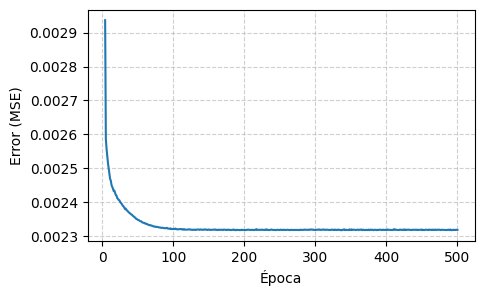
\includegraphics[width=\linewidth]{Images/error0a500.png}
        \caption{Todas las épocas}
    \end{subfigure}
    \vspace{0.55cm} % espacio vertical
    % Segunda subfigura
    \begin{subfigure}{0.65\textwidth}
        \centering
        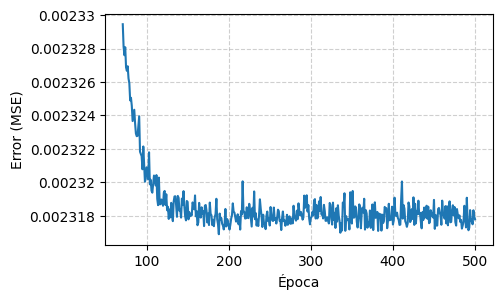
\includegraphics[width=\linewidth]{Images/error70a500.png}
        \caption{Desde la época 70.}
    \end{subfigure}
    \vspace{0.55cm}
    % Tercera subfigura
    \begin{subfigure}{0.65\textwidth}
        \centering
        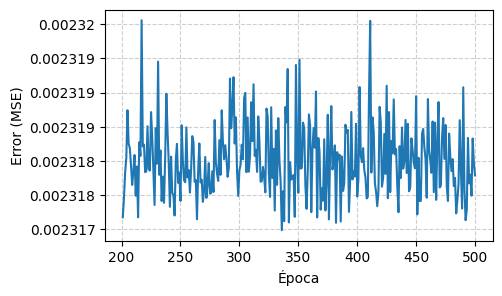
\includegraphics[width=\linewidth]{Images/error200a500.png}
        \caption{Desde la época 200.}
    \end{subfigure}
    \caption{Evolución del error de entrenamiento en función de las épocas para la configuración A15. En (a) vemos el entrenamiento completo, mientras que en (b) y (c) tenemos un acercamiento a la sección final del mismo.}
    \label{fig:tres_errores_train}
\end{figure}

En la Figura se ve claramente que primero hay una reducción rápida y pronunciada del error, indicando que el modelo aprende los patrones principales de manera eficiente. La convergencia es notablemente rápida, alcanzando valores cercanos al mínimo antes
de la época $100$. Luego, durante las épocas intermedias, el error continúa disminuyendo pero a un ritmo considerablemente menor, sugiriendo un refinamiento gradual de los pesos del modelo. Esta fase muestra la típica meseta de aprendizaje donde las mejoras incrementales requieren más tiempo de procesamiento.

En la fase final ($200$ a $500$ épocas), el error se estabiliza en valores muy bajos con fluctuaciones menores, sugiriendo que el modelo ha alcanzado un equilibrio, o al menos un mínimo local. Este patrón de convergencia parece indicar que entrenamientos tan largos, aunque garantizan convergencia completa, incluyen un número considerable de épocas redundantes. La configuración A16, idéntica pero con solo $70$ épocas, logra rendimiento prácticamente equivalente, validando esta hipótesis y demostrando la eficiencia de entrenamientos más cortos para arquitecturas bien diseñadas.

\titulito{Visualización de los filtros sobre el conjunto de test}

Vamos a mostrar ahora cómo se ven algunos de los modelos entrenados sobre imágenes del conjunto de test, el cual, recordemos, se compone de imágenes artificiales creadas de la misma manera que el dataset de entrenamiento.

En la Figura \ref{fig:imtest_A15} podemos ver el modelo A15, que es el de menor error de testeo, aplicado a una imagen.  El modelo demuestra una capacidad notable para aprender y reproducir los niveles de grises de la imagen original, logrando una reducción efectiva del ruido \emph{speckle}. Sin embargo, se observa que el autoencoder tiende a generar ciertos patrones que no están presentes en la imagen original.

\begin{figure}[htbp]
	\vspace{0.5cm}
    \centering
    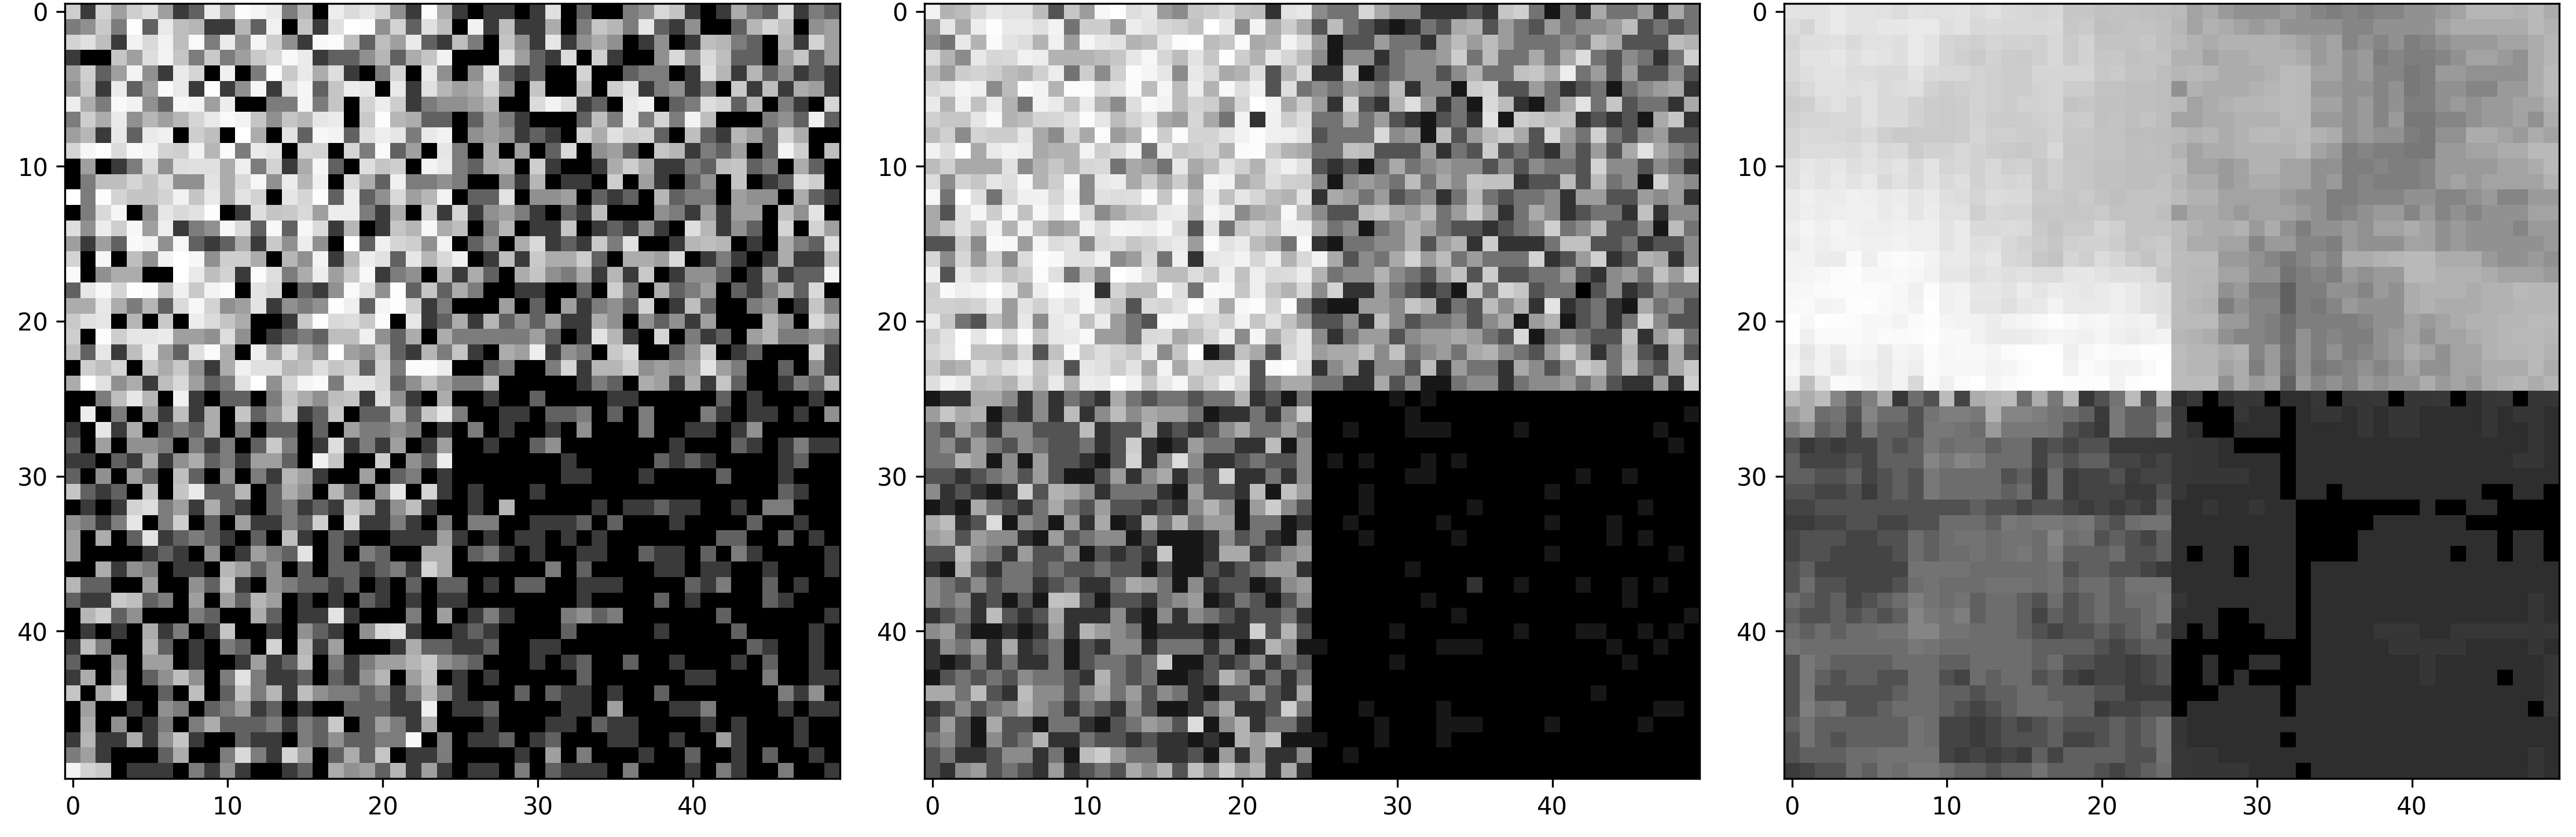
\includegraphics[height=4.5cm]{Images/imtest_A15.png}
    \caption{Imagen de ejemplo ilustrando el filtro A15 aplicado a una imagen del dataset de test. A la derecha está la imagen con ruido \emph{speckle}, la entrada de la red. En el centro está la imagen limpia, el \emph{target}. A la izquierda está la salida de la red.}
    \label{fig:imtest_A15}
\end{figure}

Este comportamiento es esperable dado que las redes convolucionales procesan la información teniendo en cuenta que la entrada es una imagen bidimensional, donde la proximidad espacial entre píxeles es un factor determinante. Esta característica hace que el modelo sea sensible a las relaciones de vecindad entre píxeles y tienda a imponer cierta estructura espacial en la reconstrucción, aunque a veces esta no exista originalmente.

La principal limitación observada es la dificultad del modelo para reconocer y preservar adecuadamente la componente aleatoria del \emph{backscatter}. Recordemos que lo describimos como una variable aleatoria con distribución $\Gamma^{-1}$. Mientras que el autoencoder maneja eficientemente los niveles de gris y las estructuras coherentes de la imagen (como los bordes entre particiones), presenta mayor dificultad para distinguir entre el ruido \emph{speckle} que debe eliminarse y la textura natural inherente al \emph{backscatter}, que debería preservarse. Queremos destacar que este comportamiento es consistente en todas las arquitecturas.

Veamos ahora en la Figura \ref{fig:imtest_A16} el ejemplo de la arquitectura A16, que es idéntica a la A15 salvo que con menos épocas de entrenamiento ($500$ épocas de A15 contra tan solo $70$ de A16). Los resultados obtenidos son notablemente similares a los del modelo A15, lo cual era esperable considerando que ambas arquitecturas presentaron errores de testeo comparables, siendo el de A15 apenas mejor.

\begin{figure}[htbp]
	\vspace{0.5cm}
    \centering
    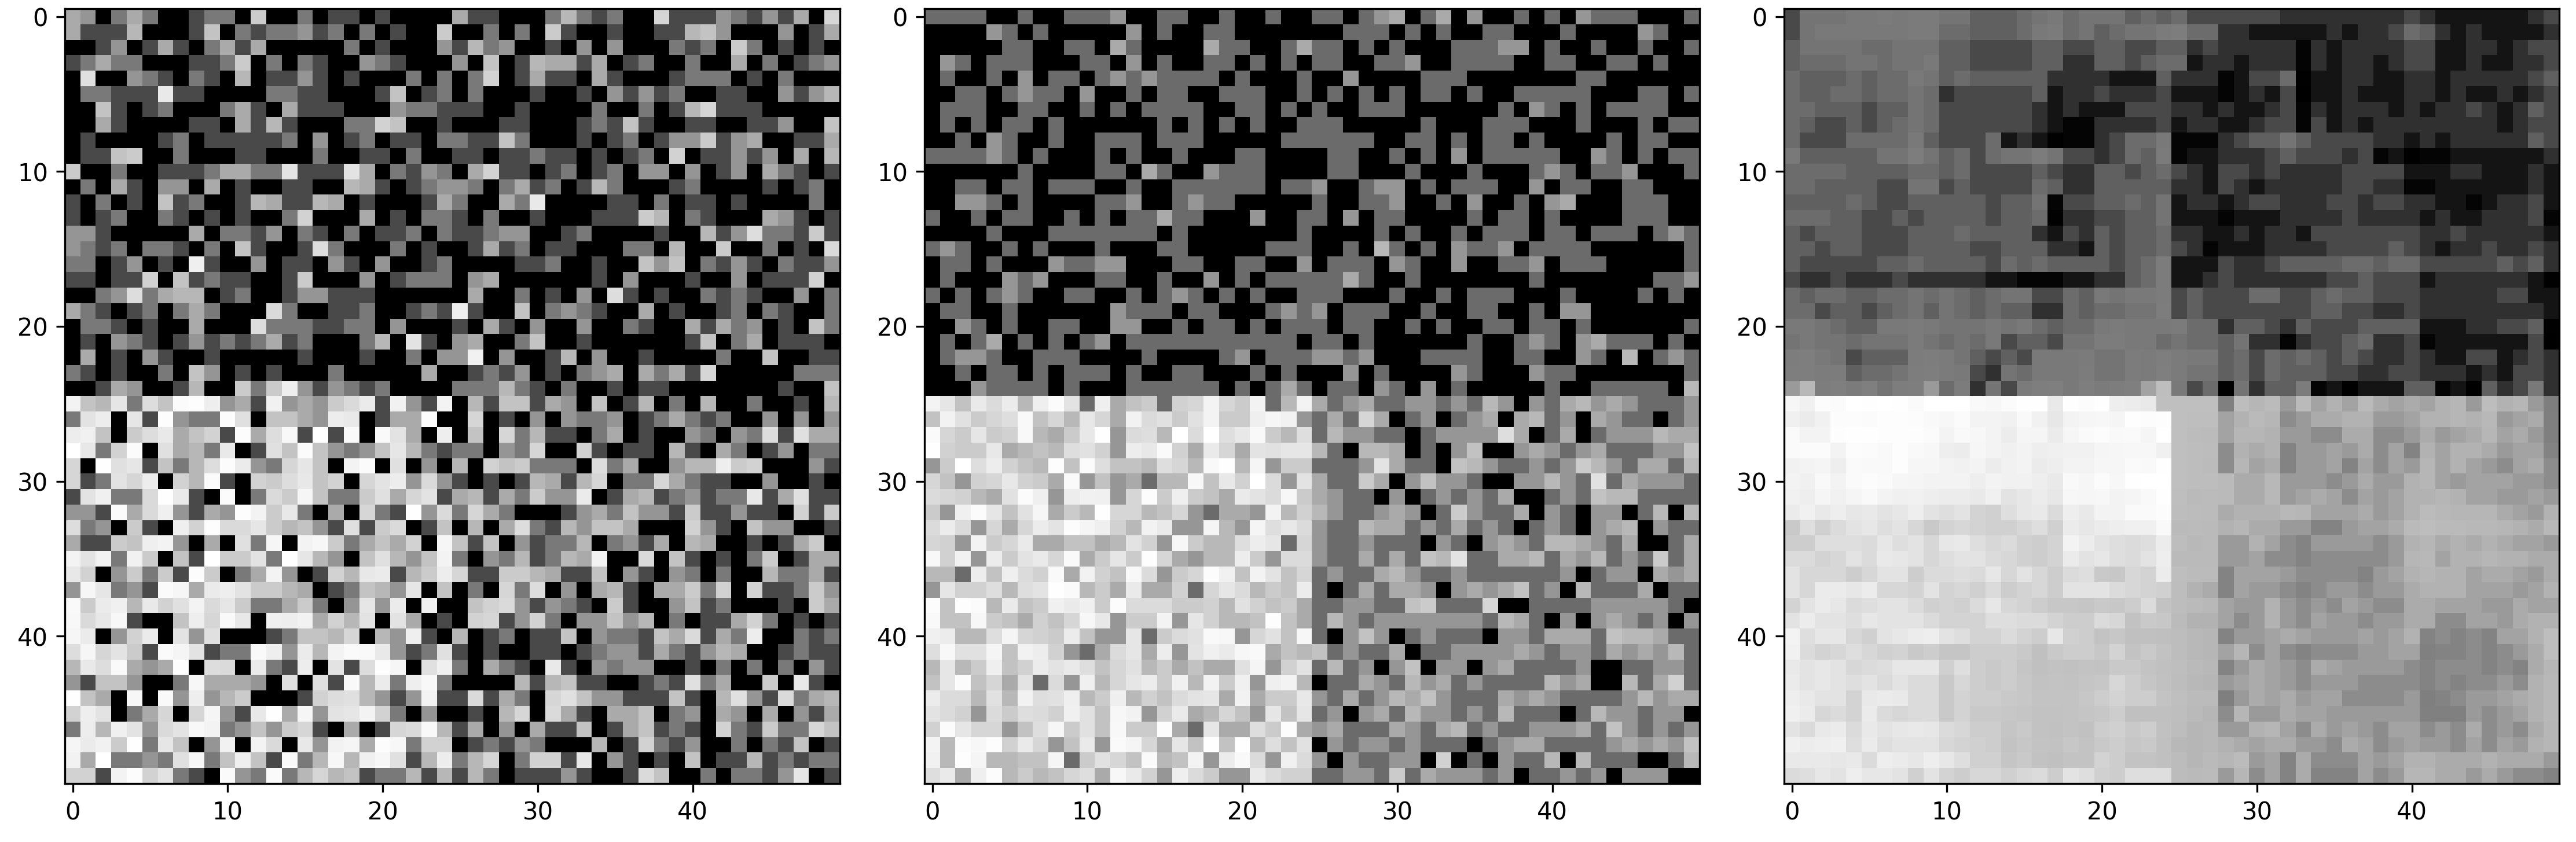
\includegraphics[height=4.5cm]{Images/imtest_A16.png}
    \caption{Imagen de ejemplo ilustrando el filtro A16 aplicado a una imagen del dataset de test. A la derecha está la imagen con ruido \emph{speckle}, la entrada de la red. En el centro está la imagen limpia, el \emph{target}. A la izquierda está la salida de la red.}
    \label{fig:imtest_A16}
\end{figure}

La principal diferencia observable radica en la calidad de las estructuras generadas en las zonas homogéneas. En el modelo A16, estas estructuras aparecen ligeramente más toscas y menos suavizadas que en A15, presentando una textura algo más irregular.

Este comportamiento sugiere que el proceso de aprendizaje del autoencoder sigue una progresión específica: durante las primeras épocas de entrenamiento (en las primeras 70, o incluso antes), el modelo adquiere rápidamente la capacidad de entender los niveles de grises y las características más evidentes de la imagen, como los bordes de las particiones. Las épocas adicionales de entrenamiento se dedican principalmente a un proceso de refinamiento, donde el autoencoder ajusta los detalles finos para generar transiciones más suaves y estructuras más regulares.

Por último, en la Figura \ref{fig:imtest_A20} tenemos una visualización de los resultados de la arquitecura A20. Elegimos esa en particular por ser una configuración que utiliza distintas particiones en su dataset de entrenamiento. De hecho, en la figura se observa el filtro aplicado a dos imágenes con particiones distintas.

\begin{figure}[htbp]
	\vspace{0.5cm}
    \centering
    
    \begin{subfigure}[b]{\textwidth}
        \centering
        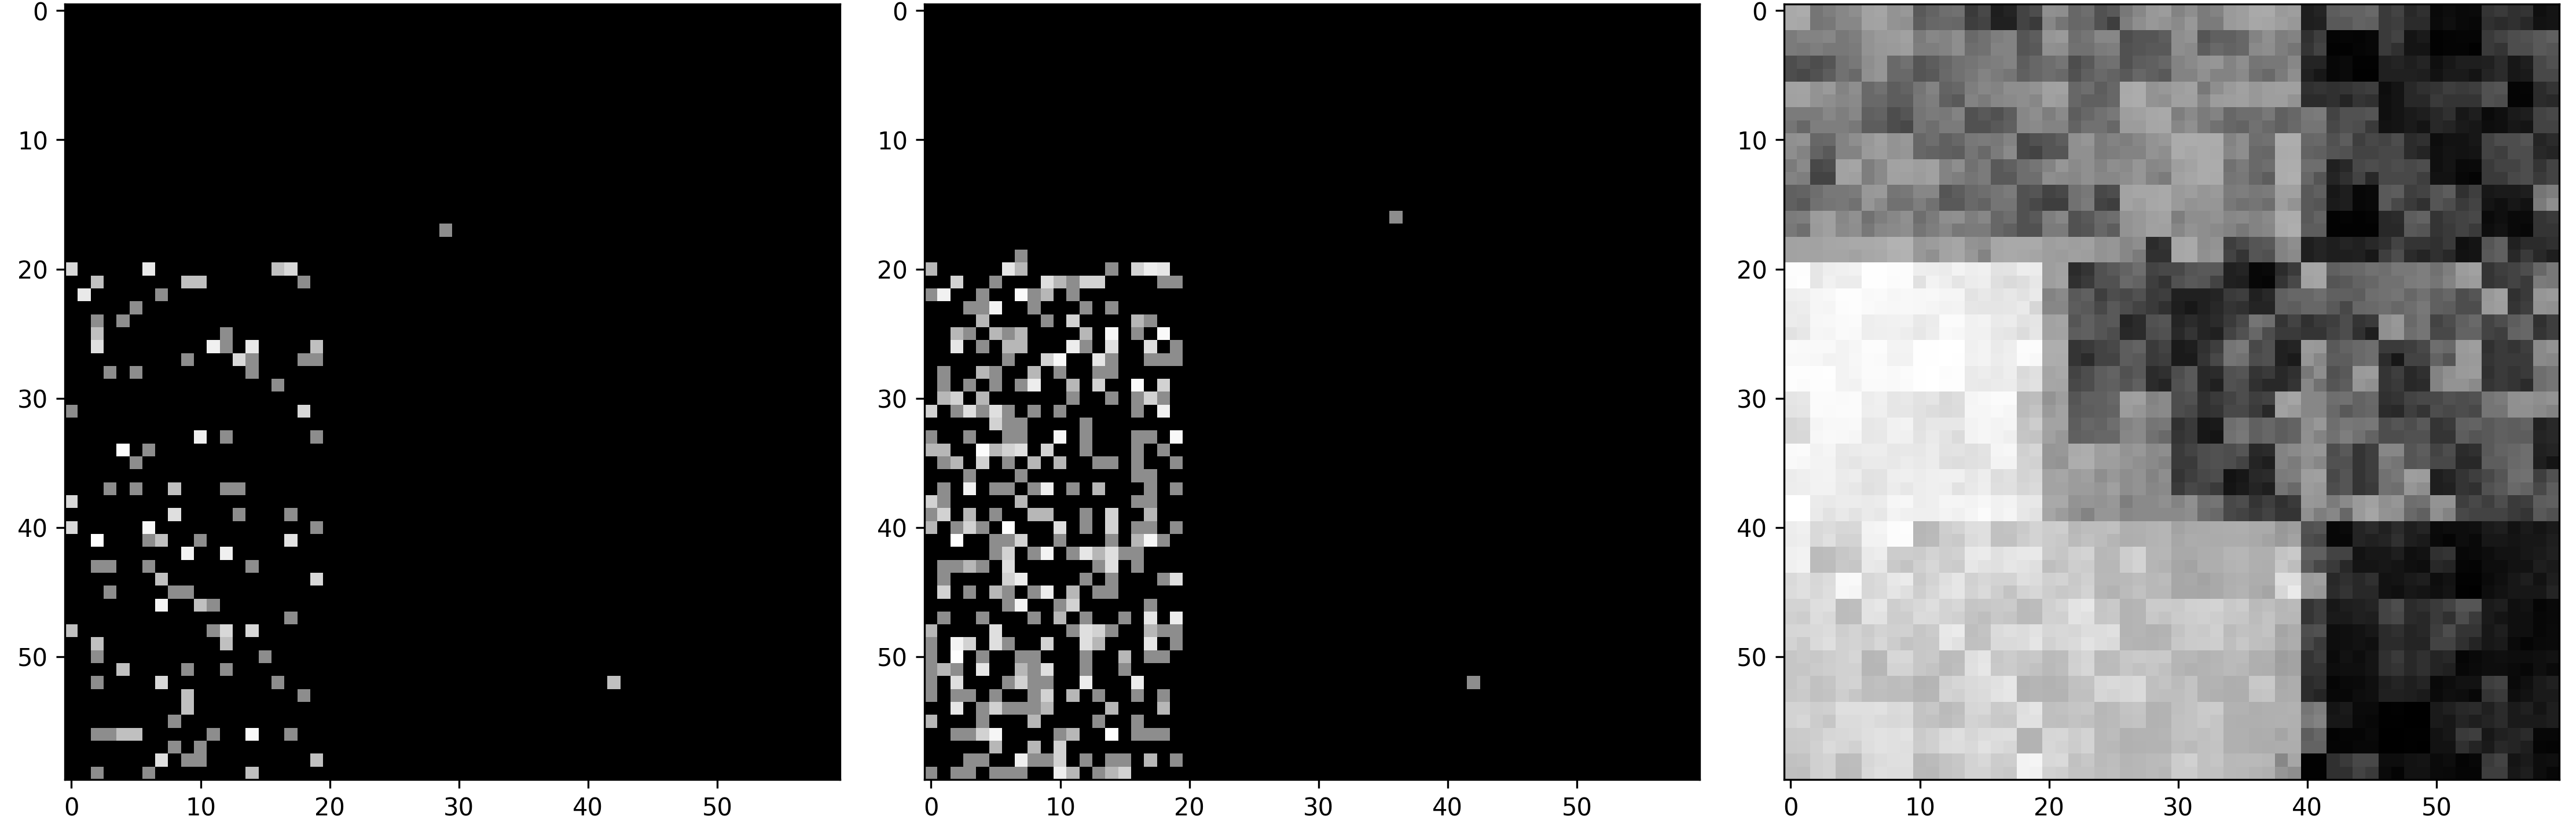
\includegraphics[width=0.86\textwidth]{Images/imtest_A20_1.png}
        \caption{Ejemplo de una imagen con partición de $3\times3$.}
        \label{fig:imtest_A20_1}
    \end{subfigure}
    
    \vspace{0.5cm} % Espacio entre las subfiguras
    
    \begin{subfigure}[b]{\textwidth}
        \centering
        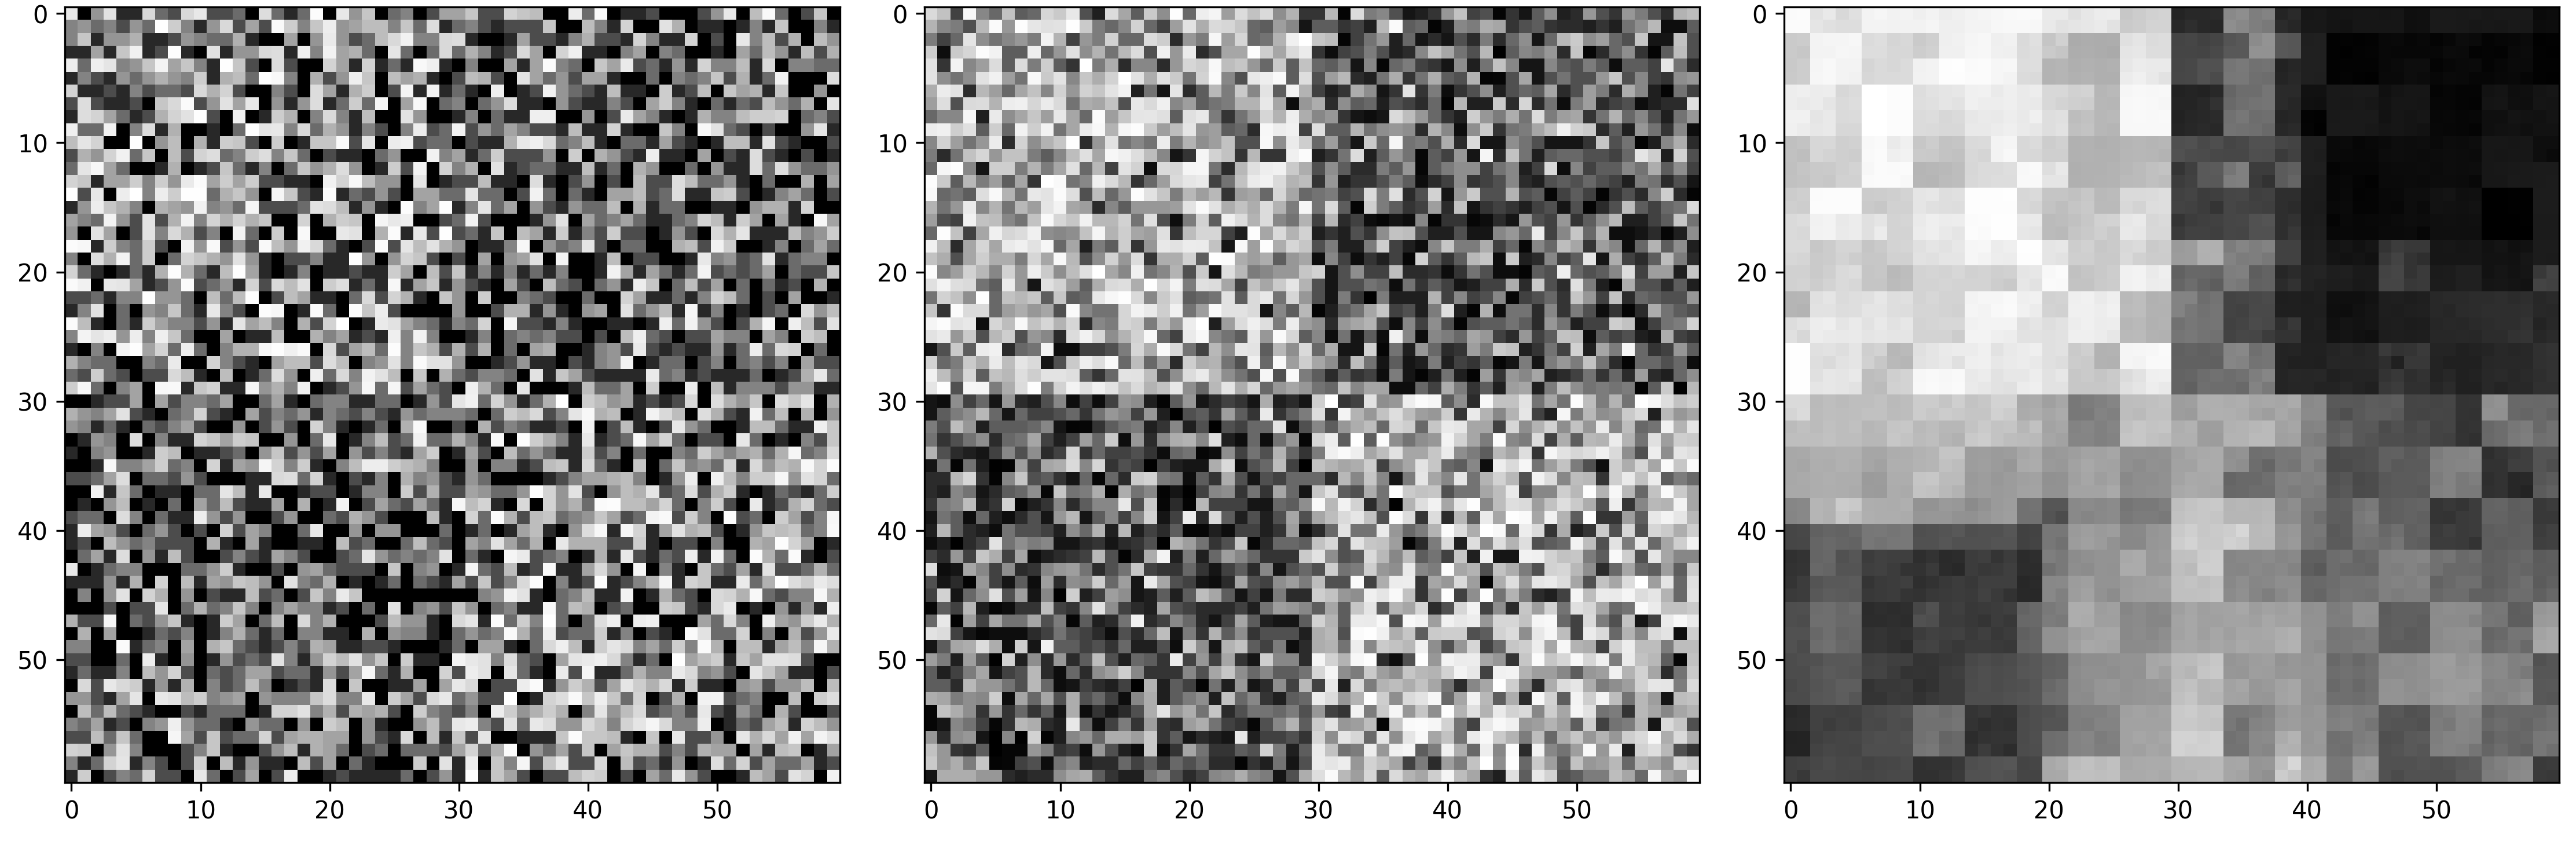
\includegraphics[width=0.86\textwidth]{Images/imtest_A20_2.png}
        \caption{Ejemplo de una imagen con partición de $2\times2$}
        \label{fig:imtest_A20_2}
    \end{subfigure}
    
    \caption{Imagenes de ejemplo ilustrando el filtro A20 aplicado a una imagen del dataset de test. Tanto en (a) como en (b), a la derecha está la imagen con ruido \emph{speckle}, la entrada de la red. En el centro está la imagen limpia, el \emph{target}. A la izquierda está la salida de la red.}
    \label{fig:imtest_A20}
\end{figure}

Visualmente podemos observar que el filtro A20 produce resultados menos prolijos que las arquitecturas A15 y A16 previamente analizadas. Las zonas que deberían presentar características homogéneas aparecen más manchadas y con mayor irregularidad en la textura, mostrando una calidad de suavizado inferior comparada con los modelos anteriores.

Sin embargo, este comportamiento es esperable, considerando que le estamos imponiendo una mayor complejidad al modelo al proporcionarle imágenes con estructuras diversas durante el entrenamiento. Esta variabilidad estructural en el dataset representa un desafío adicional para el autoencoder, que debe aprender a generalizar patrones de limpieza de ruido \emph{speckle} a través de diferentes configuraciones espaciales y características de imagen.

Esta aparente pérdida en el resultado es, en realidad, el precio que pagamos por ganar flexibilidad y capacidad de generalización. Esperamos que esta mayor robustez del modelo se traduzca en un mejor desempeño cuando se enfrente a imágenes SAR reales, cuyas estructuras son inherentemente menos organizadas y rígidas que las imágenes sintéticas utilizadas en el entrenamiento. La capacidad del modelo A20 para manejar esta diversidad estructural debería resultar en una mayor adaptabilidad a las condiciones variables y complejas presentes en datos SAR del mundo real.

\subsection{Aplicación del modelo a imágenes reales}

\begin{figure}[htbp]
	\vspace{0.1cm}
	\centering
	
	\begin{subfigure}[b]{\textwidth}
		\centering
		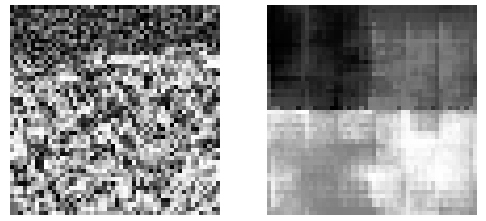
\includegraphics[width=0.67\textwidth]{Images/realimages_A15.png}
		\caption{Ejemplo para la arquitectura A15}
		\label{fig:realimages_A15}
	\end{subfigure}
	
	\vspace{0.5cm} % Espacio entre las subfiguras
	
	\begin{subfigure}[b]{\textwidth}
		\centering
		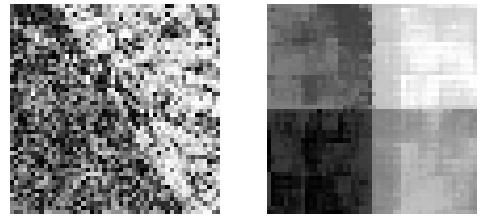
\includegraphics[width=0.67\textwidth]{Images/realimages_A16.png}
		\caption{Ejemplo para la arquitectura A16}
		\label{fig:realimages_A16}
	\end{subfigure}
	
	\vspace{0.5cm} % Espacio entre las subfiguras
	
	\begin{subfigure}[b]{\textwidth}
		\centering
		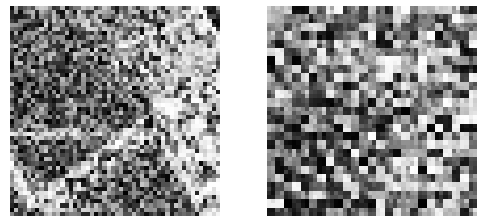
\includegraphics[width=0.67\textwidth]{Images/realimages_A20.png}
		\caption{Ejemplo para la arquitectura A20}
		\label{fig:realimages_A20}
	\end{subfigure}
	
	\caption{Ejemplos de autoencoders aplicados a imágenes SAR reales. Las imágenes de la izquierda son las imágenes SAR, las de la derecha son los resultados de cada modelo.}
	\label{fig:modelosclasicos_imreales}
\end{figure}

Para evaluar el desempeño de los autoencoders convolucionales en condiciones más realistas, los aplicamos a imágenes SAR reales, en particular a las que se muestran en la Figura \ref{fig:imagenes_sar_ruido}. Este experimento nos permite analizar cómo se comportan los modelos cuando no operan sobre imágenes del conjunto de testeo, que fueron generadas artificialmente manteniendo la misma estructura del dataset de entrenamiento. En otras palabras, buscamos evaluar qué sucede cuando los modelos se enfrentan a condiciones distintas de aquellas para las que fueron optimizados.

Dado que las imágenes de la Figura \ref{fig:imagenes_sar_ruido} presentan dimensiones mayores a $50\times50$ píxeles, mientras que todos nuestros autoencoders fueron entrenados con imágenes de $50\times50$, procedimos a extraer secciones aleatorias de $50\times50$ píxeles de las imágenes reales para luego aplicar los autoencoders sobre estas regiones. Presentamos los resultados obtenidos para las arquitecturas A15, A16 y A20, las mismas cuyos resultados analizamos en la Sección anterior. Estos resultados se muestran en la Figura \ref{fig:modelosclasicos_imreales}.

Para las arquitecturas A15 y A16 observamos resultados cualitativamente similares. Lo que se evidencia claramente es que estas configuraciones aprendieron las particiones específicas con las cuales fueron entrenadas. Esto no constituye necesariamente un caso de sobreajuste, sino que probablemente se deba a que todas las imágenes observadas durante el entrenamiento presentaban este tipo de particionado. Además, el hecho de que A16, que es idéntica a A15 pero con menor número de épocas de entrenamiento, presente el mismo comportamiento, refuerza la hipótesis de que no se trata de \emph{overfitting}. No obstante, podemos observar que los cuadrantes respetan en líneas generales los niveles de gris de la imagen SAR original: en las zonas donde la imagen original es más oscura, el cuadrante correspondiente también presenta tonalidades más oscuras, y viceversa. Pareciera que el autoencoder promedia el nivel de gris dentro de cada cuadrante. Todo esto demuestra que, si bien estas arquitecturas obtuvieron errores de test muy bajos, cuando se las evalúa sobre imágenes reales que no poseen la misma estructura que su dataset de entrenamiento, no logran generalizar adecuadamente y su desempeño se degrada significativamente.

En contraste, A20 fue entrenada con diferentes particiones de imágenes, lo cual resultó en un error de test superior, dado que el conjunto de datos es más complejo y, por lo tanto, más difícil de aprender para la red. Sin embargo, su desempeño sobre imágenes SAR reales es claramente mejor. Esto confirma que efectivamente la exposición a distintas particiones durante el entrenamiento ayudó al modelo a generalizar y desempeñarse mejor en imágenes reales. Aunque el resultado visual no es óptimo y carece de mucho detalle, se respetan mejor las estructuras de la imagen original y no presenta el problema de las particiones tan marcadamente.

Otra cuestión relevante a considerar es la cantidad de looks de las imágenes reales utilizadas. En particular, la imagen de Múnich (Figura \ref{Munich}) presenta $L=1$, mientras que la de San Francisco (Figura \ref{Sanfran}) posee $L=3$. Dado que todos nuestros modelos fueron entrenados con $L=1$, la comparación más apropiada debería realizarse con la imagen de Múnich. No obstante, en ambos casos se observaron resultados cualitativos muy similares.

El hecho de que los resultados sobre imágenes reales no hayan sido completamente satisfactorios nos indica que es conveniente considerar el entrenamiento utilizando imágenes reales. Además nos sugiere que la estrategia de entrenar con particiones impone una restricción demasiado severa al modelo, limitando su capacidad de generalización. En consecuencia, en el siguiente capítulo exploraremos la alternativa de entrenar las redes neuronales directamente con imágenes SAR reales.

\subsection{Métodos estadísticos de medición de la calidad del filtro}

Como se explicó en la Sección \ref{sec:metodos_stat}, otra forma de medir la bondad de los filtros es utilizando los métodos estadísticos de primer y segundo orden.

Con respecto al método de primer orden, recordemos que se basa en la imagen ratio entre la imagen de salida de la red y la imagen original ruidosa. Un buen filtro produciría una imagen ratio sin estructura. Un ejemplo de estas imágenes se observa en la Figura \ref{fig:im_ratios}, donde se aprecia que la imagen ratio no presenta prácticamente ninguna estructura, lo cual es positivo e implica que contiene solamente ruido, como era de esperarse.

En cuanto al método de segundo orden, se basa en el hecho de que un buen filtro produciría valores similares del coeficiente de homogeneidad si permutamos la matriz de Haralick obtenida a partir de nuestra imagen. Para calcular esto utilizaremos 30 permutaciones.

Los resultados de ambos filtros se presentan en la Tabla \ref{tab:statistics_results}, donde se muestran los valores del filtro de primer y segundo orden, junto con la suma de ambos, la cual denominamos $\mathcal{M}$.

\vspace{1cm}

\begin{figure}[htbp]
	\vspace{0.2cm}
	\centering
	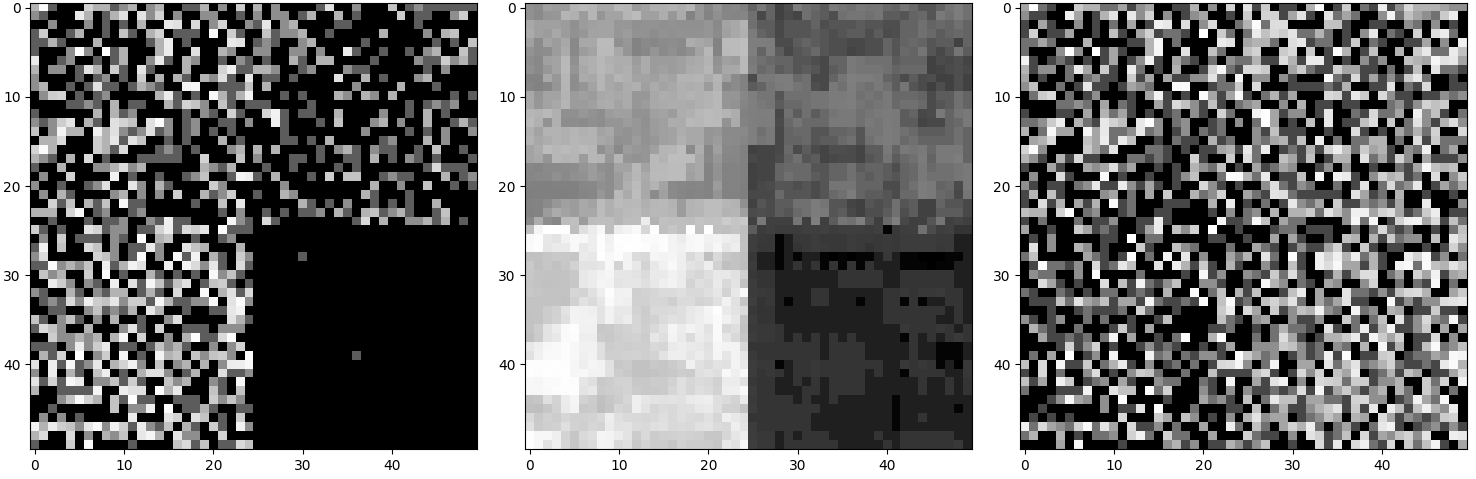
\includegraphics[height=4.5cm]{Images/im_ratios.png}
	\caption{La imagen de la izquierda es una imagen con ruido \emph{speckle} obtenida artificialmente, es decir, con distribución \( \mathcal{G}_I^0 \). La del medio es la imagen que sale del autoencoder. La de la derecha es la imagen ratio que se obtiene al dividir punto a punto la de la izquierda por la del medio.}
	\label{fig:im_ratios}
\end{figure}

Las configuraciones con los mejores estadísticos fueron A24, A2 y A22, ocupando las primeras tres posiciones en el ranking con valores de $\mathcal{M}$ de $2.576$, $3.206$ y $3.414$ respectivamente. Notemos que estas configuraciones no presentaron los errores de test más bajos de la tabla, sino que se ubicaron en posiciones intermedias (ranking $1$, $2$ y $3$ en estadísticos vs. $7$, $13$ y $17$ en errores de test). Lograron valores bajos en los estadístico de primer y segundo orden (A24: $0.233$ y $2.343$; A2: $0.218$ y $2.988$; A22: $0.232$ y $3.182$), lo que indica un buen desempeño. A24 se destaca por su bajo valor de $\delta_h$.

Un hallazgo particularmente interesante es el comportamiento de la configuración A15, que ocupó el primer lugar en términos de error de test más bajo ($0.002318$ MSE) y mostró una excelente capacidad de generalización (tan solo $0.04\%$ de aumento entre los errores de train y test). Sin embargo, esta misma configuración se ubica en la posición $9$ del ranking estadístico con $\mathcal{M} = 3.768$. Este fenómeno sugiere que un bajo error de reconstrucción no necesariamente garantiza un buen desempeño en las métricas estadísticas.

Vemos por ejemplo que las configuraciones A4, A6 y A20 presentaron signos claros de overfitting con aumentos significativas entre los errores de train y test ($28.51\%$, $29.18\%$ y $20.19\%$ respectivamente). Coherentemente, estas configuraciones mostraron estadísticos subóptimos, ocupando las posiciones $13$, $20$ y $19$ en el ranking con valores de $\mathcal{M}$ de $4.111$, $7.506$ y $5.289$. Esto confirma que el \emph{overfitting} no solo afecta la capacidad de generalización sino también la calidad del filtrado en términos de preservación de propiedades estadísticas.

Los modelos A6, A5 y A21 tienen los peores estadísticos ($\mathcal{M}$ = $7.506$, $7.787$ y $8.003$ respectivamente), junto con un pobre desempeño en el error de test (ranking $19$, $18$ y $21$ respectivamente). Otra vez, esto muestra cierta correspondencia entre las tablas \ref{tab:testing_results} y \ref{tab:statistics_results}.

\begin{table}[htbp]
	\hspace{0.2cm}
	\centering
	\caption{Resultados de los estadísticos de primer ($r_{\text{ENL},\mu}$) y segundo orden ($\delta_h$) para cada configuración, junto con la suma de ambos ($\mathcal{M}$). Se ordenan de menor a mayor valor de $\mathcal{M}$.\newline}
	\label{tab:statistics_results}
	\small
	\begin{tabular}{|c|c|c|c|c|}
		\hline
		\textbf{Ranking} &
		\textbf{Config.} &
		\makecell{$r_{\text{ENL},\mu}$} &
		\makecell{$\delta_h$} &
		$\mathcal{M}$ \\
		\hline
		1 & A24 & 0.233 & 2.343 & 2.576 \\
		2 & A2 & 0.218 & 2.988 & 3.206 \\
		3 & A22 & 0.232 & 3.182 & 3.414 \\
		4 & A25 & 0.241	& 3.273	& 3.515 \\
		5 & A16 & 0.201 & 3.329 & 3.530 \\
		6 & A10 & 0.207 & 3.340 & 3.548 \\
		7 & A14 & 0.204 & 3.402 & 3.606 \\
		8 & A11 & 0.238 & 3.453 & 3.691 \\
		9 & A15 & 0.194 & 3.574 & 3.768 \\
		10 & A8 & 0.222 & 3.629 & 3.851 \\
		11 & A13 & 0.213 & 3.687 & 3.900 \\
		12 & A18 & 0.230 & 3.873 & 4.103 \\
		13 & A4 & 0.273 & 3.838 & 4.111 \\
		14 & A9 & 0.217 & 3.963 & 4.179 \\
		15 & A17 & 0.313 & 3.979 & 4.293 \\
		16 & A12 & 0.236 & 4.232 & 4.468 \\
		17 & A7 & 0.208 & 4.291 & 4.499 \\
		18 & A23 & 0.305 & 4.688 & 4.993 \\
		19 & A20 & 0.343 & 4.946 & 5.289 \\
		20 & A6 & 0.643 & 6.863 & 7.506 \\
		21 & A5 & 0.344 & 7.443 & 7.787 \\
		22 & A21 & 0.376 & 7.627 & 8.003 \\
		\hline
		- & A1 & - & - & - \\
		- & A3 & - & - & - \\
		- & A19 & - & - & - \\
		\hline
	\end{tabular}
	\vspace{0.5cm}
	\begin{flushleft}
		\footnotesize
		\textbf{Nota:}
		Para las configuraciones A1 y A19 no se pudieron calcular los estadísticos por problemas de convergencia. El modelo A3 ya aclaramos que no pudo entrenarse.
	\end{flushleft}
\end{table}

Es importante destacar que las configuraciones A1, A3 y A19 no pudieron ser evaluadas debido a problemas de convergencia durante el entrenamiento. En el caso particular de A3, el modelo no pudo entrenarse por la gran cantidad de parámetros entrenables que posee, como ya habíamos mencionado. Mientras que A1 y A19 presentaron problemas de convergencia que impidieron el cálculo de los estadísticos correspondientes.

\subsection{Comparación con otros filtros}

\titulito{Métodos desarrollados en otros trabajos}

\vspace{0.2cm}

En el trabajo de Chan et al. \cite{chan2022entropy} se desarrollan otros métodos de limpieza de imágenes SAR, y se comparan los estadísticos de primer y segundo orden para varios de estos métodos. Al contrastar nuestros resultados con los obtenidos por Chan et al., observamos que sus valores son efectivamente menores. No para el estadístico de primer orden, sino para el de segundo orden ($\delta_h$​), donde métodos como \emph{Shannon Entropy} y \emph{Renyi Entropy} alcanzan valores de $0.113$ y $0.173$ respectivamente, comparados con nuestros mejores resultados de $2.343$ para A24.

Sin embargo, debemos destacar que las imágenes utilizadas en el trabajo de Chen et al. son diferentes a las empleadas en nuestros experimentos, lo que hace que la comparación directa de los estadísticos no sea completamente válida. Las características específicas del conjunto de imágenes utilizadas para testear y como fueron construidas pueden influir en los valores absolutos de estos estadísticos.

Lo que resulta más relevante de esta comparación es que nuestros estadísticos se encuentran en el mismo orden de magnitud que los reportados por Chan et al., lo que valida que nuestros métodos están operando en rangos comparables a los del estado del arte. Por tanto, nos enfocamos más en la consistencia relativa entre nuestras configuraciones y en la correlación entre el rendimiento durante el entrenamiento y la calidad del filtrado, que en la comparación absoluta con valores obtenidos sobre conjuntos de datos diferentes.

\vspace{0.3cm}

\titulito{Filtro de Lee}

\vspace{0.2cm}

Otra forma de contextualizar el rendimiento de nuestros autoencoders convolucionales es realizando una comparación con el filtro de Lee, uno de los métodos clásicos y conocidos para limpieza de imágenes.

\begin{figure}[htbp]
	\vspace{0.2cm}
	\centering
	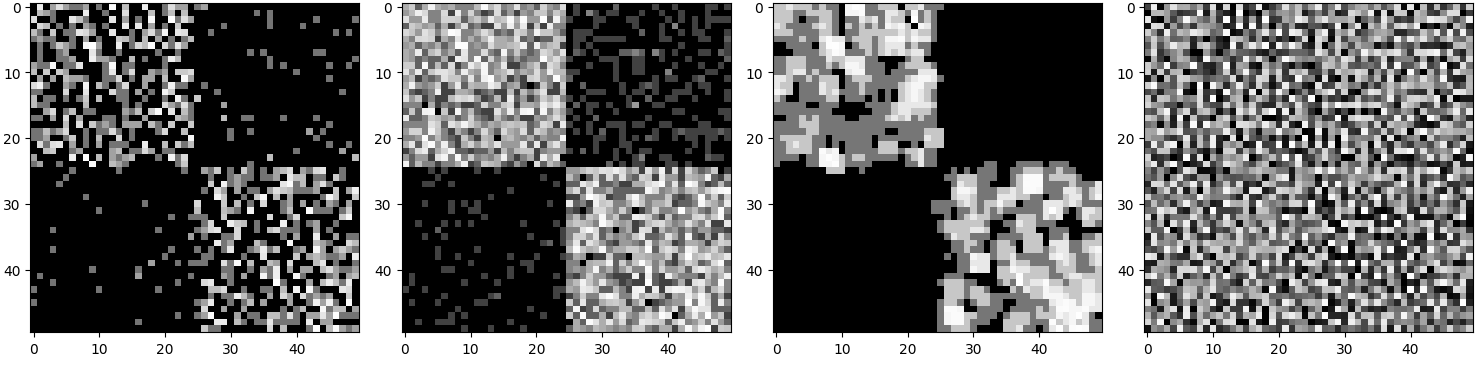
\includegraphics[height=3.4cm]{Images/ejemplo_filtro_lee.png}
	\caption{Ejemplo del funcionamiento del filtro de Lee. La primera imagen es una imagen artificial con ruido \emph{speckle}. La segunda es su correspondiente imagen limpia. La tercera es el resultado de aplicar el filtro de Lee a la imagen original, con tamaño de ventana de $3$ píxeles. La cuarta es el ratio punto a punto entre la imagen ruidosa y la filtrada.}
	\label{fig:filtro_lee}
\end{figure}

En cuanto a la metodología de comparación, generamos un dataset artificial siguiendo la misma técnica empleada anteriormente para el entrenamiento de nuestros modelos. Implementamos el filtro de Lee con una ventana de $3\times3$ píxeles, aunque recordemos que este valor debe elegirlo el usuario y afecta los resultados finales. Para obtener una estimación de la varianza del ruido, parámetro que debemos pasarle al filtro de Lee, seleccionamos regiones homogéneas en las imágenes originales y calculamos la varianza local en estas zonas. Posteriormente, promediamos estos valores de varianza sobre múltiples imágenes del conjunto de datos para obtener una estimación robusta de este parámetro.

Aplicamos el filtro de Lee sobre las imágenes contaminadas con ruido speckle artificial y calculamos el ratio entre las imágenes ruidosas y las imágenes filtradas, siguiendo el mismo protocolo utilizado para evaluar nuestros autoencoders. En la Figura \ref{fig:filtro_lee} vemos un ejemplo de una imagen procesada por el filtro Lee junto a la imagen ratio. Podemos ver que el filtro genera resultados visuales satisfactorios, aunque presenta problemas en los bordes y pierde un poco del detalle y la granularidad que tiene la imagen limpia. Por otra parte, es difícil distinguir estructuras en la imagen ratio, lo cual es signo de un buen filtro.

A partir de todo lo anterior, computamos los estadísticos de primer orden y segundo orden sobre todo el conjunto de imágenes, promediando los resultados para obtener valores únicos que permitan una comparación directa con las arquitecturas que desarrollamos. Obtuvimos lo siguiente:

\begin{itemize}
	\item Estadístico de primer orden ($r_{\text{ENL},\mu}$) = $0.399$
	\item Estadístico de segundo orden ($\delta_h$) = $4.654$
	\item $\mathcal{M} = r_{\text{ENL},\mu} + \delta_h = 5.053$
\end{itemize}

Podemos ver que los valores están dentro del rango de los que obtuvimos para nuestros modelos, pero cercano a los que peor desempeño tuvieron. Con lo cual podemos afirmar que gran parte de nuestros modelos performan mejor que el filtro de Lee en esta tarea, usando estas métricas como referencia. De cualquier forma, es importante destacar que el objetivo de esta comparación no es necesariamente demostrar que nuestros autoencoders superan al filtro de Lee en todos los casos, sino más bien verificar que nuestros métodos compiten en el mismo rango de rendimiento que este método clásico bien establecido.

Para mesurar el efecto del tamaño de ventana en el filtro, en la Tabla \ref{tab:lee_ventanas}  vemos los resultados del filtro de Lee para valores de ventana de variados. De allí queda claro que el error empeora con el tamaño, y que la elección de una ventana de $3\times3$ es la que ofrece un mejor funcionamiento.

\begin{table}[htbp]
	\hspace{0.2cm}
	\centering
	\caption{Resultados del filtro de Lee para distintos tamaños de ventana. Se muestran los estadísticos de primer ($r_{\text{ENL},\mu}$) y segundo orden ($\delta_h$), junto con la suma de ambos ($\mathcal{M}$).\newline}
	\label{tab:lee_ventanas}
	\small
	\begin{tabular}{|c|c|c|c|}
		\hline
		\textbf{Tamaño ventana} &
		\makecell{$r_{\text{ENL},\mu}$} &
		\makecell{$\delta_h$} &
		$\mathcal{M}$ \\
		\hline
		3\times3 & 0.399 & 4.654 & 5.053 \\
		5\times5 & 0.448 & 8.331 & 8.819 \\
		7\times7 & 0.509 & 10.837 & 11.346 \\
		\hline
	\end{tabular}
\end{table}

Esta comparación es particularmente valiosa porque el filtro de Lee ha sido ampliamente validado en la literatura y utilizado en aplicaciones prácticas durante décadas. Por tanto, demostrar que nuestras arquitecturas de \emph{deep learning} pueden alcanzar estadísticos comparables confirma la viabilidad de este enfoque para el problema de \emph{despeckling}, especialmente considerando las ventajas adicionales que pueden ofrecer los métodos basados en redes neuronales, como la adaptabilidad a diferentes tipos de imágenes y la capacidad de aprender patrones complejos directamente de los datos.

\section{Modelos entrenados con imágenes reales}

Los experimentos previos con modelos entrenados utilizando imágenes artificiales muestran limitaciones significativas en su aplicación a imágenes reales. Observamos que estos modelos tienden a aprender las particiones específicas de las imágenes sintéticas, lo que compromete su capacidad de generalización cuando se enfrenta a imágenes con estructuras diferentes a las presentes en el conjunto de datos de entrenamiento. Esta característica representa una barrera para la aplicabilidad práctica de los modelos que desarrollamos.

\begin{table}[htbp]
	\centering
	\caption{Resumen de las cinco arquitecturas de redes convolucionales diseñadas para el  entrenamiento con imágenes SAR reales.}
	\label{tab:imreales_configs}
	\small
	\begin{tabular}{|c|c|c|c|c|c|c|}
		\hline
		\textbf{Config.} & \textbf{Capas Conv.} & \textbf{\emph{Encoding Dim.}} & \textbf{Épocas} & \begin{tabular}[c]{@{}c@{}}\textbf{Tamaño} \\ \textbf{Img.}\end{tabular}\ & \textbf{LR} & \textbf{\emph{Scheduler}} \\
		\hline
		\hline
		\multicolumn{7}{|c|}{\textbf{Arquitecturas con capas densas}} \\
		\hline
		Config B1 & \begin{tabular}[c]{@{}c@{}}2 Conv. \\ \emph{Flatten} \\ 2 Densas \\ \emph{Unflatten}\\ 2 Conv2DT.\end{tabular} & 1600 & 300 & $512\times512$ & 0.001 & \begin{tabular}[c]{@{}c@{}}ELR \\ ($\gamma=0.95$)\end{tabular} \\
		\hline
		\hline
		\multicolumn{7}{|c|}{\textbf{Arquitecturas completamente convolucionales}} \\
		\hline
		Config B2 & \begin{tabular}[c]{@{}c@{}}5 Conv. \\ 5 Conv2DT.\end{tabular} & 1500 & 300 & $256\times256$ & 0.001 & \begin{tabular}[c]{@{}c@{}}ELR \\ ($\gamma=0.97$)\end{tabular} \\
		\hline
		Config B3 & \begin{tabular}[c]{@{}c@{}}6 Conv. \\ 6 Conv2DT.\end{tabular} & 1500 & 200 & $256\times256$ & 0.001 & \begin{tabular}[c]{@{}c@{}}ELR \\ ($\gamma=0.97$)\end{tabular} \\
		\hline
		Config B4 & \begin{tabular}[c]{@{}c@{}}4 Conv. \\ 4 Conv2DT.\end{tabular} & 1500 & 200 & $128\times128$ & 0.001 & \begin{tabular}[c]{@{}c@{}}ELR \\ ($\gamma=0.97$)\end{tabular} \\
		\hline
		\hline
		\multicolumn{7}{|c|}{\textbf{Arquitecturas con otras técnicas}} \\
		\hline
		Config B5 & \begin{tabular}[c]{@{}c@{}}2 Conv. \\ \emph{MaxPool} \\ Conv. \\ \emph{MaxPool} \\ Conv. \\ Conv2DT. \\ \emph{Upsample} \\ Conv2DT. \\ \emph{Upsample} \\ 2 Conv2DT.\end{tabular} & 1500 & 200 & $256\times256$ & 0.001 & \begin{tabular}[c]{@{}c@{}}ELR \\ ($\gamma=0.9999$)\end{tabular} \\
		\hline
	\end{tabular}
\end{table}

\begin{table}[htbp]
	\centering
	\caption{Resultados para los modelos entrenados con imágenes SAR reales. Vemos el error de testeo para cada configuración (ordenados por rendimiento), y el error de entrenamiento en la última época. También se muestra la variación del primero con respecto al segundo. Este valor es verde cuando la variación es negativa y rojo cuando es positiva.}
	\label{tab:testing_imreal_results}
	\small
	\begin{tabular}{|c|c|c|c|c|}
		\hline
		\textbf{Ranking} &
		\textbf{Config.} &
		\makecell{\textbf{Error de} \\ \textbf{\emph{test} (MSE)}} &
		\makecell{\textbf{Error de \emph{train} (MSE)} \\ \textbf{en la última época}} &
		\makecell{\textbf{Error de \emph{test}} \\ \textbf{vs. \emph{train}}} \\
		\hline
		1 & B5 & 0.00887 & 0.00923 & \textcolor{verdecito}{$\searrow 3.900325\%$} \\
		2 & B2 & 0.00905 & 0.01007 & \textcolor{verdecito}{$\searrow 10.1290\%$} \\
		3 & B3 & 0.00907 & 0.01016 & \textcolor{verdecito}{$\searrow 10.7283\%$} \\
		4 & B4 & 0.01014 & 0.01148 & \textcolor{verdecito}{$\searrow 11.67247\%$} \\
		5 & B1 & 0.03217 & 0.00959 & \textcolor{red}{$\nearrow 235.45\%$} \\
		\hline
	\end{tabular}
\end{table}

Con el objetivo de intentar superar estas limitaciones, implementamos un enfoque de entrenamiento basado en imágenes SAR reales. Como detallamos en la Sección \ref{sec:train_real_images}, esta estrategia fue posible gracias a un conjunto de datos de acceso libre que contenía pares de imágenes SAR reales y sus correspondientes versiones limpias. La metodología empleada para obtener las imágenes limpias consistía en tomar múltiples imágenes ruidosas de la misma región, y atenuar el ruido \emph{speckle} promediandolas. La Figura \ref{fig:dataset_sar} ilustra un ejemplo representativo de estos pares de imágenes utilizadas en el entrenamiento.

Para el desarrollo experimental, diseñamos e implementamos cinco arquitecturas de redes neuronales convolucionales diferentes, cuyas características principales y configuraciones se resumen en la Tabla \ref{tab:imreales_configs}.

\begin{figure}[htbp]
	%\vspace{0.5cm}
	\centering
	
	\begin{subfigure}[b]{\textwidth}
		\centering
		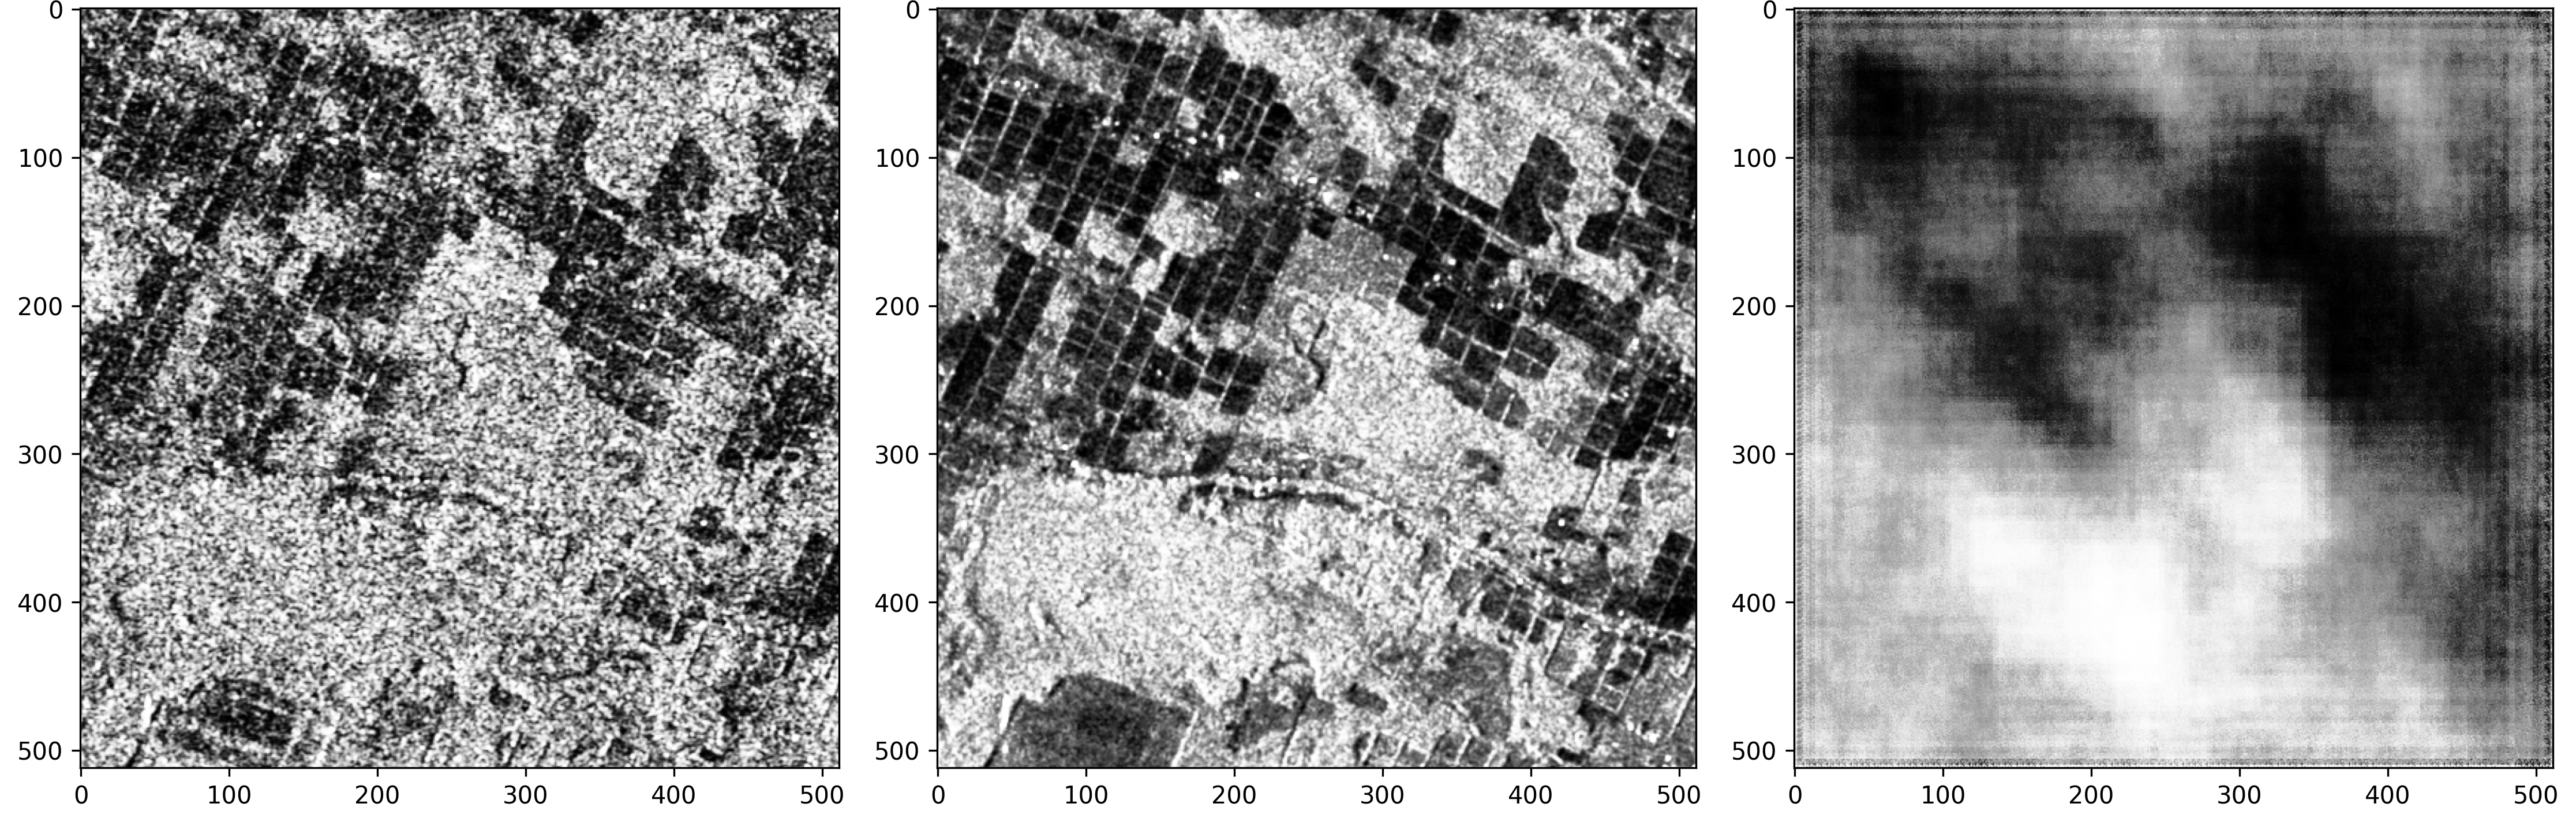
\includegraphics[width=0.95\textwidth]{Images/B1_imej_1.png}
		\caption{Primer ejemplo}
		\label{fig:B1_1}
	\end{subfigure}
	
	\vspace{0.5cm} % Espacio entre las subfiguras
	
	\begin{subfigure}[b]{\textwidth}
		\centering
		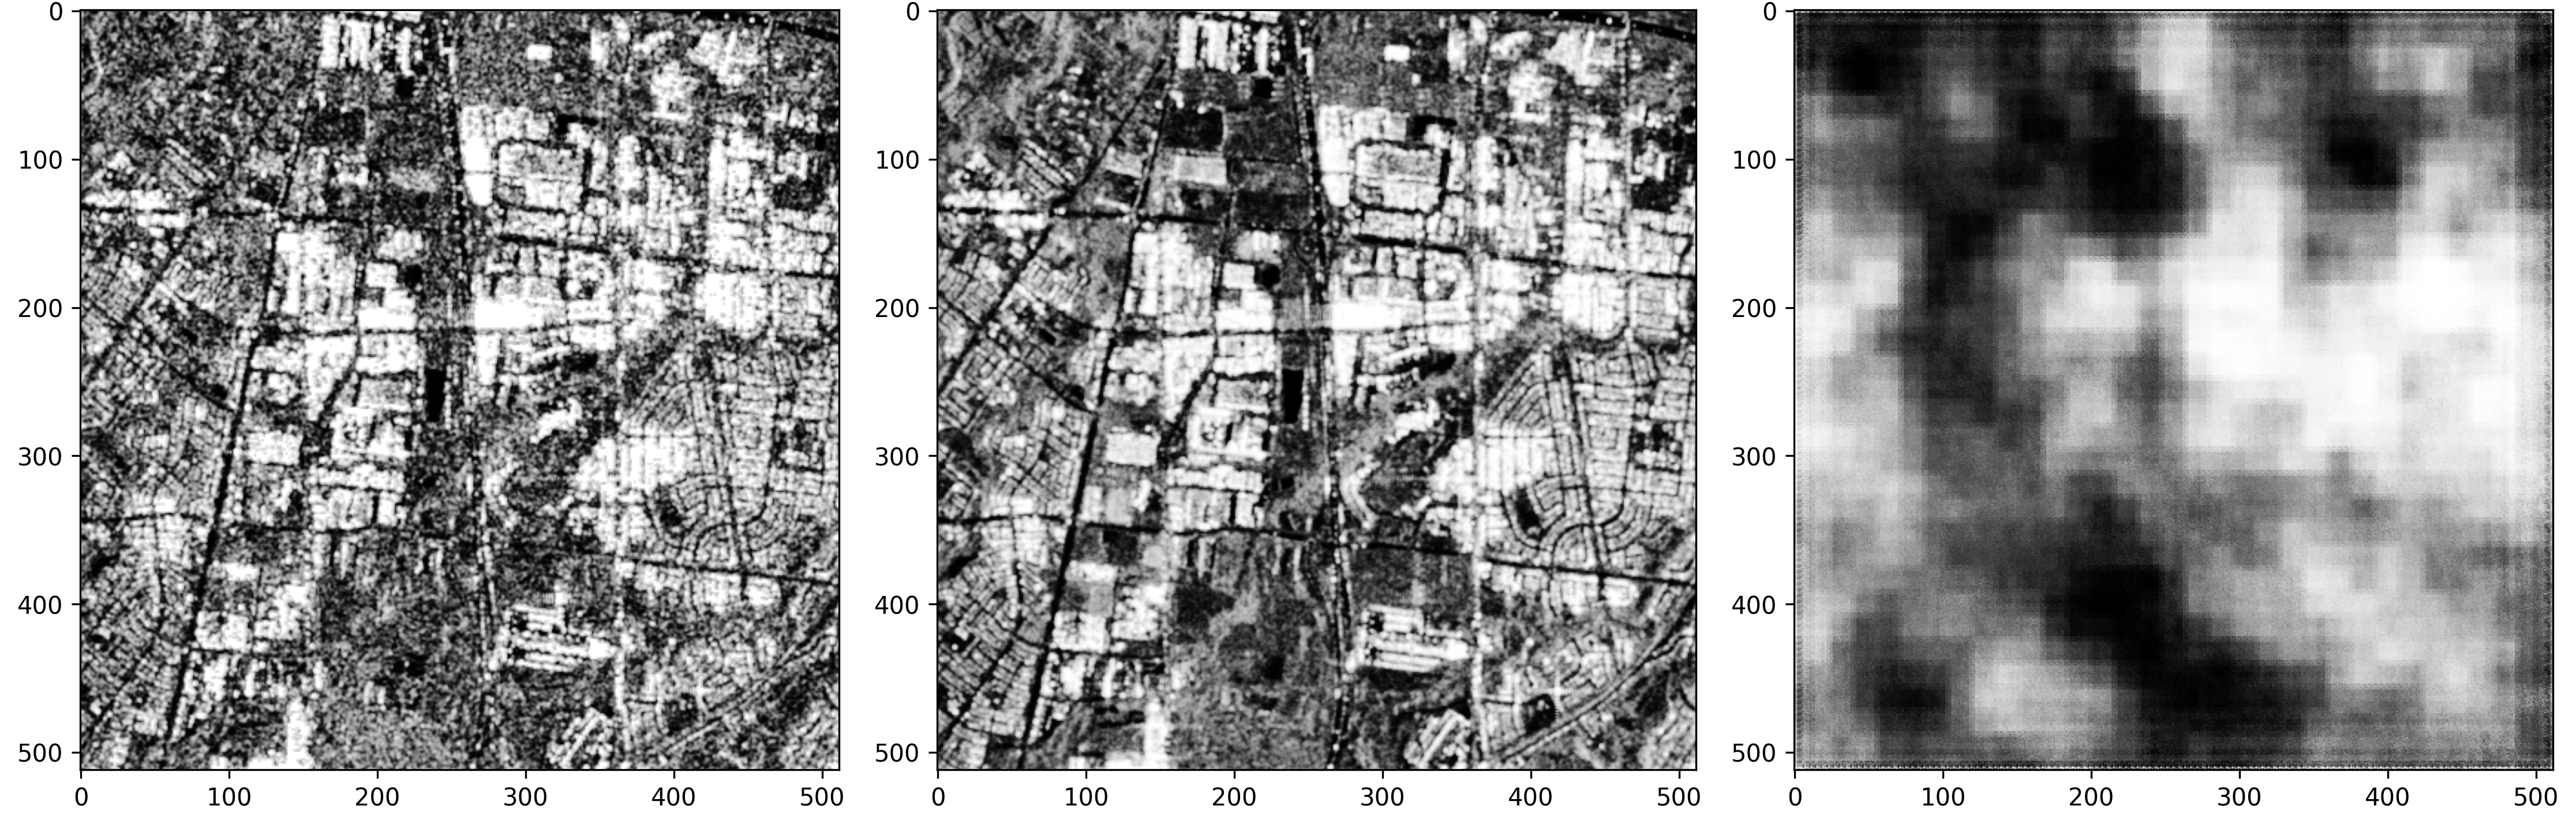
\includegraphics[width=0.95\textwidth]{Images/B1_imej_2.png}
		\caption{Segundo ejemplo}
		\label{fig:B1_2}
	\end{subfigure}
	
	\caption{Dos ejemplos de imágenes SAR reales procesadas por el modelo B1. A la izquierda la imagen SAR ruidosa, en el centro está la imagen limpia (el \emph{target} de la red), y a la derecha la salida del modelo.}
	\label{fig:B1}
\end{figure}

El dataset de entrenamiento proporciona $1500$ imágenes con una resolución de $512\times512$ píxeles. Pero trabajar con imágenes tan grandes genera redes con más parámetros entrenables de los que podemos manejar con nuestros recursos. Por eso decidimos cortarlas en subimágenes cuadradas de lado \emph{S}. Cada configuración especifica un valor para \emph{S}, el cual puede verse en la quinta columna de la Tabla \ref{tab:imreales_configs}. Implementamos entonces un procedimiento de segmentación automática para adaptar las imágenes originales a los requerimientos de cada modelo. Este consiste en extraer de manera ordenada todas las subimágenes de tamaño \emph{S}\times\emph{S} que puedan ser contenidas completamente dentro de cada imagen original de $512\times512$, y sin que haya superposición entre las subimágenes. Este enfoque permite maximizar el aprovechamiento de los datos disponibles generando múltiples muestras de entrenamiento a partir de cada imagen del dataset original.

\begin{figure}[htbp]
	%\vspace{0.5cm}
	\centering
	
	\begin{subfigure}[b]{\textwidth}
		\centering
		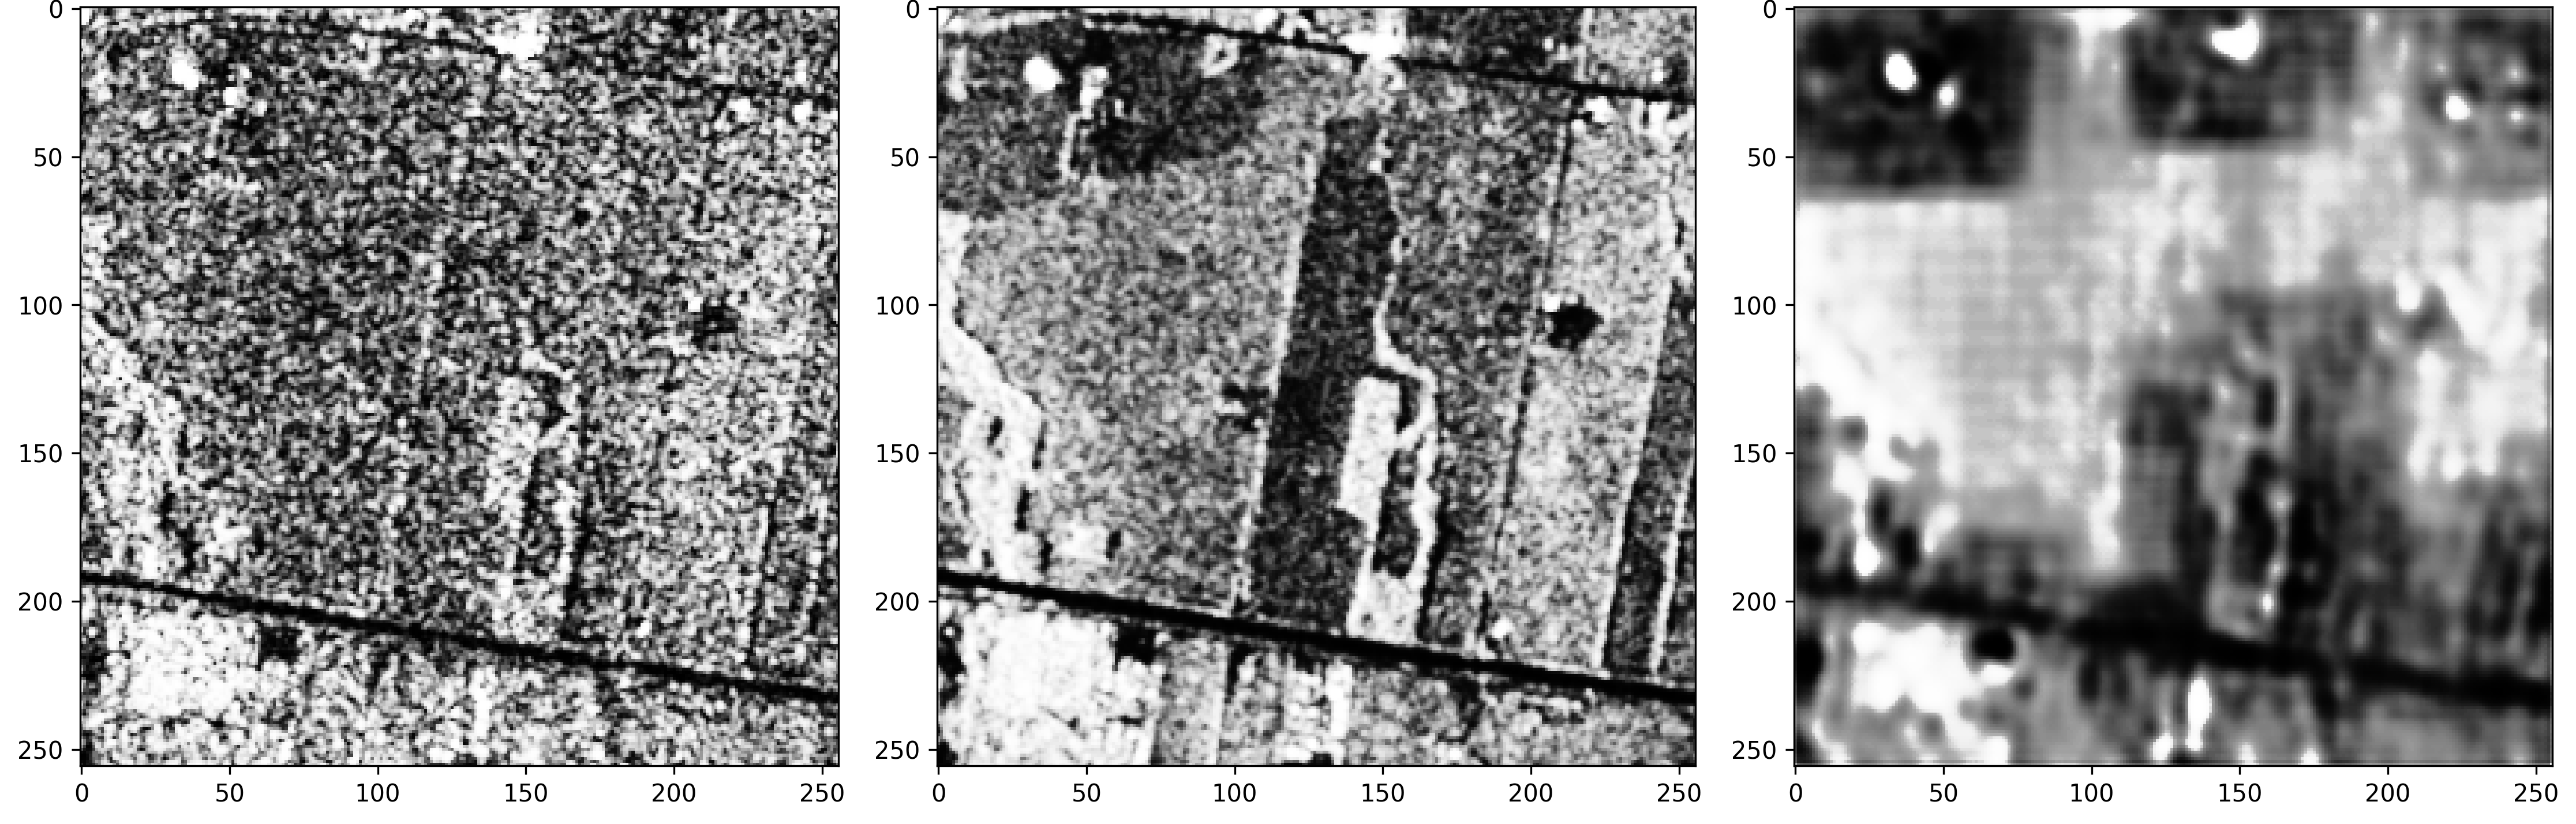
\includegraphics[width=0.95\textwidth]{Images/B3_imej_1.png}
		\caption{Primer ejemplo}
		\label{fig:B3_1}
	\end{subfigure}
	
	\vspace{0.5cm} % Espacio entre las subfiguras
	
	\begin{subfigure}[b]{\textwidth}
		\centering
		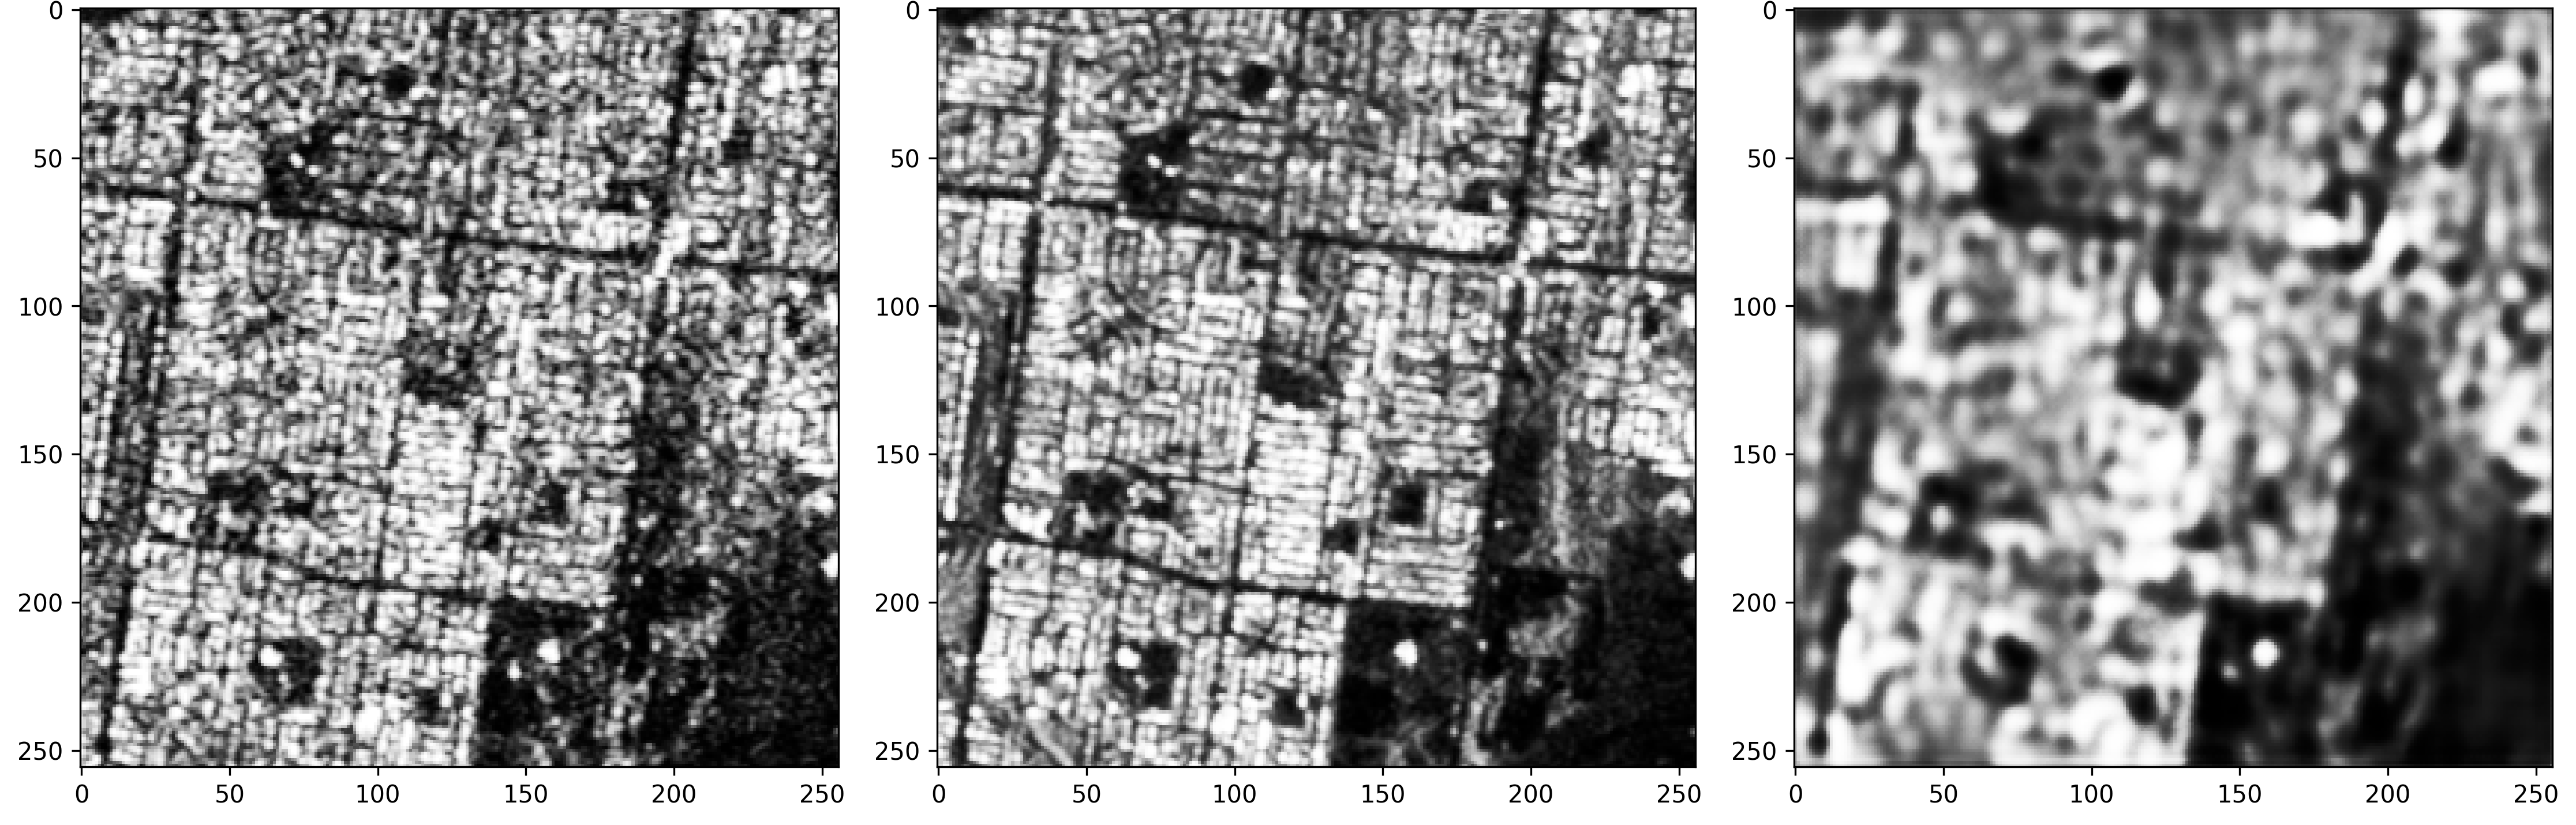
\includegraphics[width=0.95\textwidth]{Images/B3_imej_2.png}
		\caption{Segundo ejemplo}
		\label{fig:B3_2}
	\end{subfigure}
	
	\caption{Dos ejemplos de imágenes SAR reales procesadas por el modelo B3. A la izquierda la imagen SAR ruidosa, en el centro está la imagen limpia (el \emph{target} de la red), y a la derecha la salida del modelo.}
	\label{fig:B3}
\end{figure}

Como etapa de filtrado, descartamos automáticamente todas las subimágenes cuyo valor máximo de intensidad sea igual al valor mínimo, ya que éstas corresponden a regiones completamente planas sin información útil. Esta situación puede presentarse cuando el proceso de segmentación extrae secciones pequeñas de áreas uniformes dentro de las imágenes de mayor tamaño, resultando en parches que carecen de variabilidad de intensidad y, por tanto, de contenido informativo relevante para el entrenamiento.

\begin{figure}[htbp]
	%\vspace{0.5cm}
	\centering
	
	\begin{subfigure}[b]{\textwidth}
		\centering
		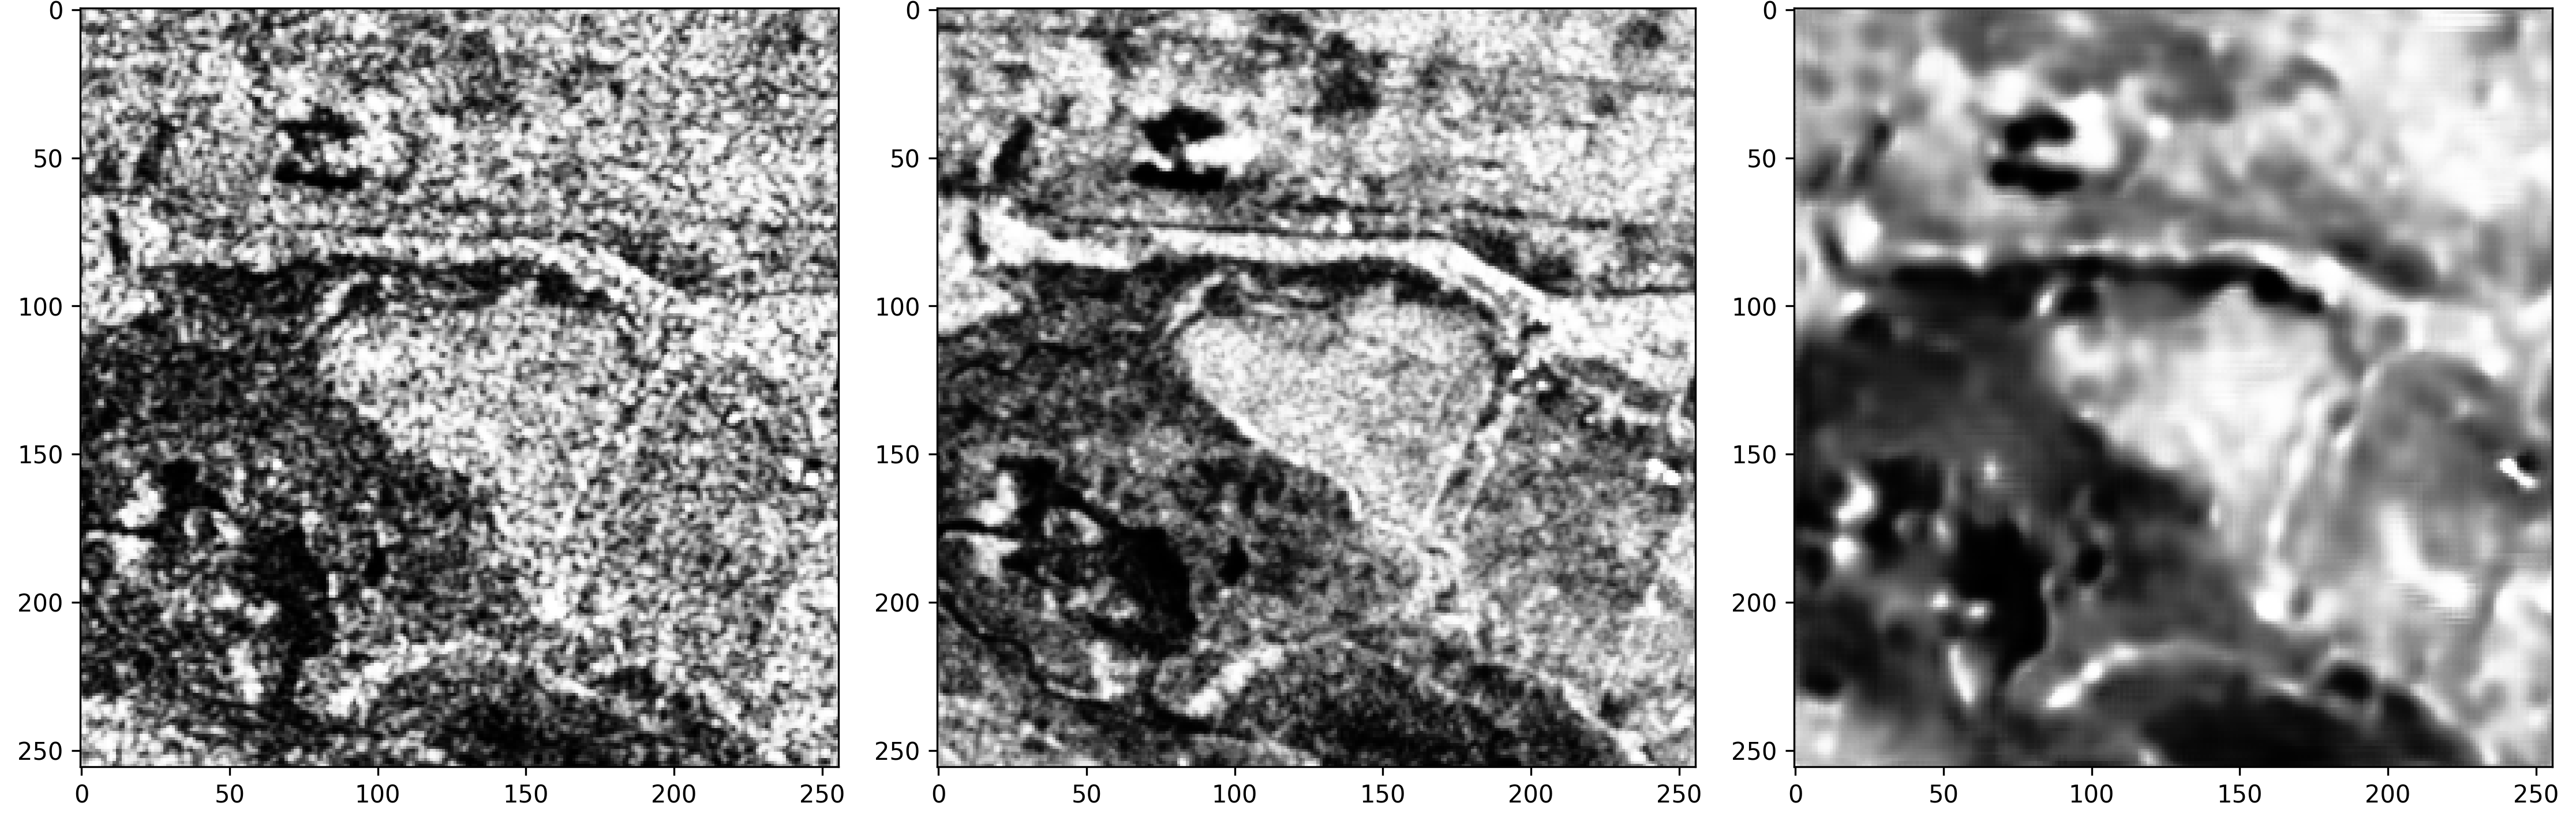
\includegraphics[width=0.95\textwidth]{Images/B5_imej_1.png}
		\caption{Primer ejemplo}
		\label{fig:B5_1}
	\end{subfigure}
	
	\vspace{0.5cm} % Espacio entre las subfiguras
	
	\begin{subfigure}[b]{\textwidth}
		\centering
		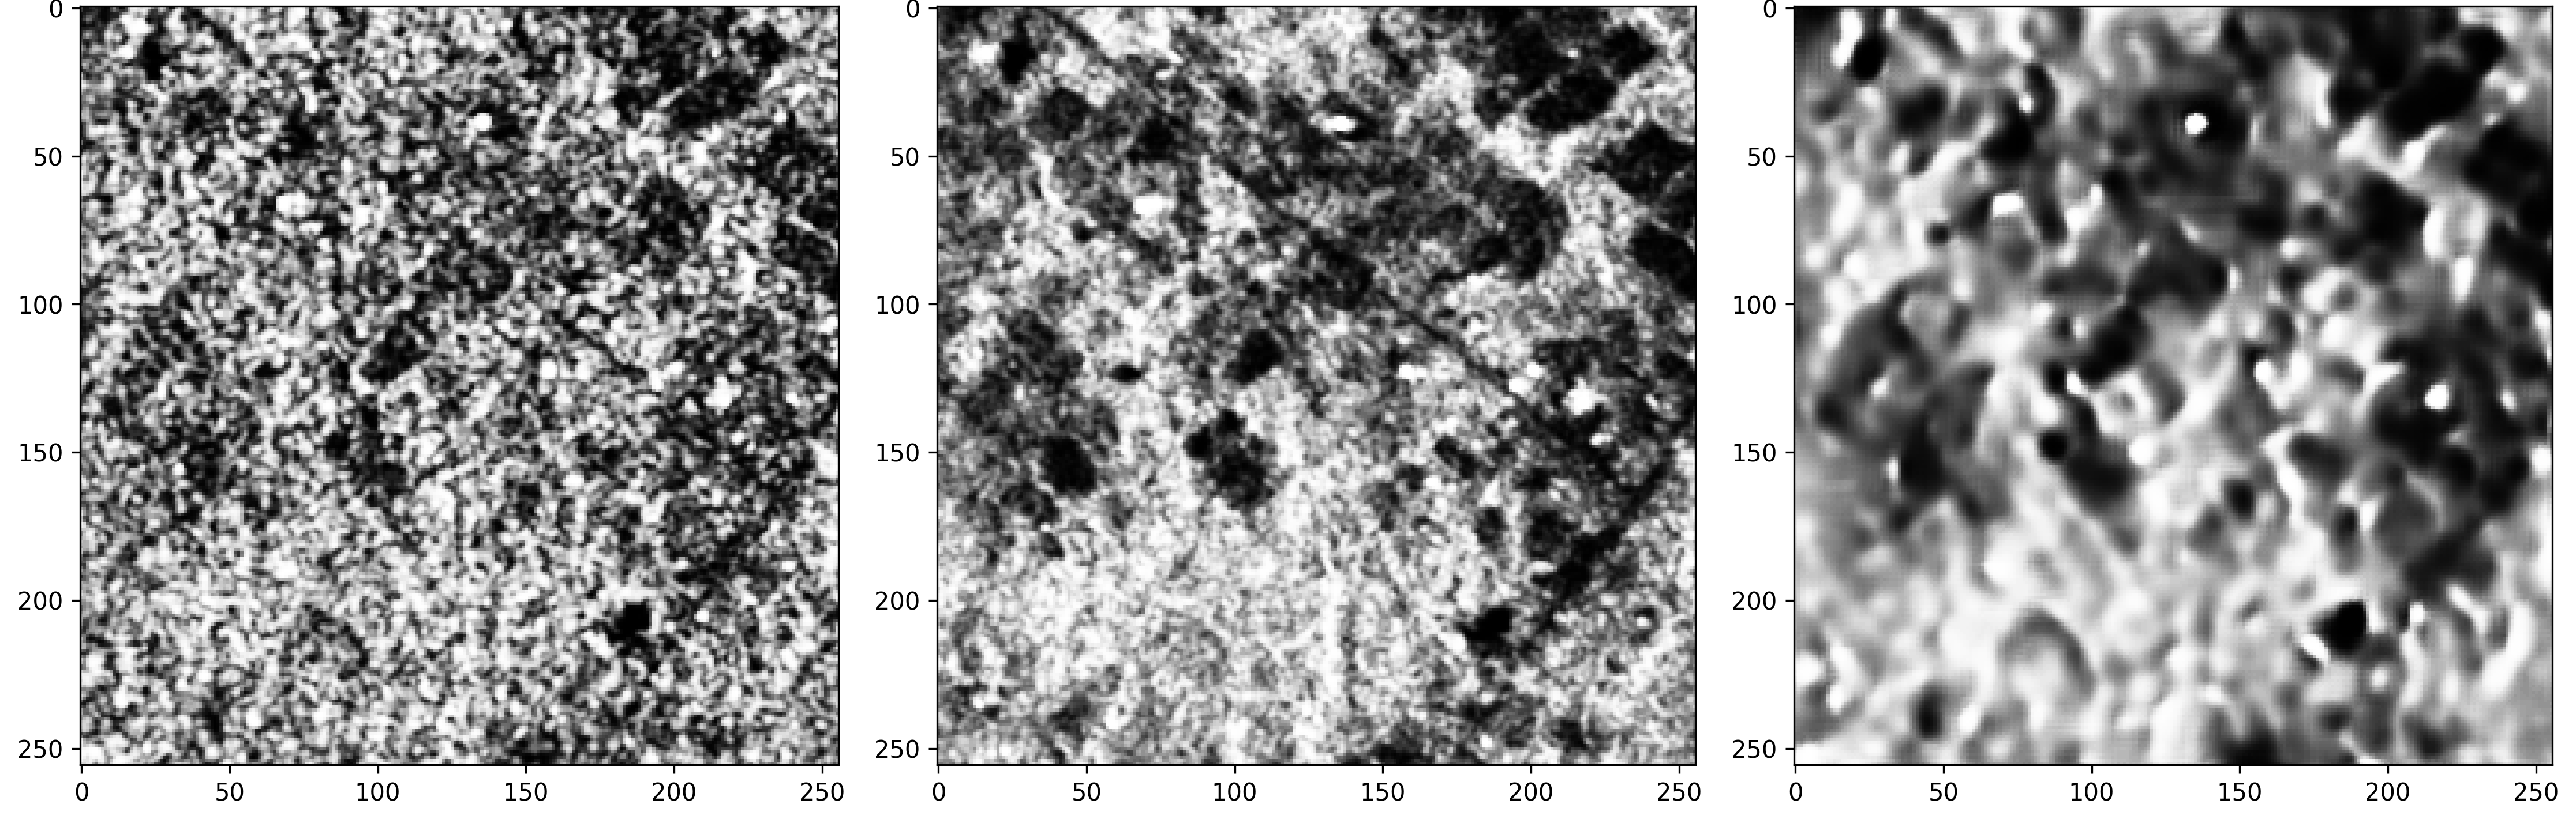
\includegraphics[width=0.95\textwidth]{Images/B5_imej_2.png}
		\caption{Segundo ejemplo}
		\label{fig:B5_2}
	\end{subfigure}
	
	\caption{Dos ejemplos de imágenes SAR reales procesadas por el modelo B5. A la izquierda la imagen SAR ruidosa, en el centro está la imagen limpia (el \emph{target} de la red), y a la derecha la salida del modelo.}
	\label{fig:B5}
\end{figure}

En todas las arquitecturas utilizamos MSE como función de pérdida y Adam como optimizador. En cuanto a las funciones de activación, en las capas intermedias empleamos ReLU o \emph{Leaky} ReLU según la configuración específica, mientras que en la capa final utilizamos siempre la función sigmoidea. Por otro lado, el tamaño de lote se fijó en $64$ muestras en todos los casos.

\vspace{1cm}

\titulito{Errores de entrenamiento y de test}

En la Tabla \ref{tab:testing_imreal_results} presentamos los resultados de entrenamiento y de test para cada arquitectura evaluada. Del análisis de los resultados observamos que la arquitectura B5 fue la que mejor desempeño mostró, sin presentar signos evidentes de \emph{overfitting}. Por otra parte, resulta llamativo que las arquitecturas B2, B3 y B4 todas exhiben un error de testeo significativamente menor al de entrenamiento, lo que sugiere un comportamiento poco convencional. Por el contrario, la configuración B1 presenta un claro caso de sobreajuste, donde el error de test es un orden de magnitud superior al de entrenamiento.

En las Figuras \ref{fig:B1}, \ref{fig:B3} y \ref{fig:B5} mostramos dos ejemplos para cada configuración, donde visualizamos cómo quedan las imágenes del conjunto de test después de ser procesadas por los respectivos autoencoders. Aquí vemos claramente cómo el modelo B1 es el más pobre en términos de reconstrucción, donde solo se divisan sombras difusas con alguna estructura vagamente similar a la imagen \emph{target}. El modelo presenta una capacidad muy limitada para capturar los detalles espaciales y las texturas características de las imágenes SAR.

En el caso de B3, cuyo error de test es considerablemente mejor, las imágenes reconstruidas ya aparecen mucho más claras y las estructuras están más definidas. Podemos distinguir con mayor claridad los elementos urbanos, las calles y los diferentes tipos de cobertura del suelo. La mejora respecto a B1 es substancial, tanto en términos de nitidez como de preservación de la información estructural.

Para B5, que representa nuestro mejor modelo, el resultado no difiere dramáticamente de B3, pero sí observamos mejoras notables en aspectos específicos. Los bordes aparecen más marcados y definidos, hay mayor fidelidad en las formas que se quieren reproducir, y se preservan mejor los detalles finos de las estructuras pequeñas como pueden ser las zonas urbanas. Particularmente, notamos una mejor reconstrucción de las características lineales como caminos y límites entre diferentes tipos de cobertura del suelo.

\titulito{Métodos estadísticos para medir la bondad del filtro}

Para poder cuantificar la calidad de los modelos de otra forma que no sea solamente el error de testeo, calculamos los estadísticos de primer y segundo orden. En ambos casos necesitamos la imagen ratio que se obtiene al dividir, píxel por píxel, la imagen de entrada por la de salida. Cuanto mejor sea el filtro, la imagen ratio presentará menos estructuras y será más similar a una imagen de puro rudio. En la Figura \ref{fig:ratios_imreales} vemos ejemplos de imágenes ratio para algunos de los modelos que diseañmos.

\begin{figure}[htbp]
	%\vspace{0.5cm}
	\centering
	
	\begin{subfigure}[b]{\textwidth}
		\centering
		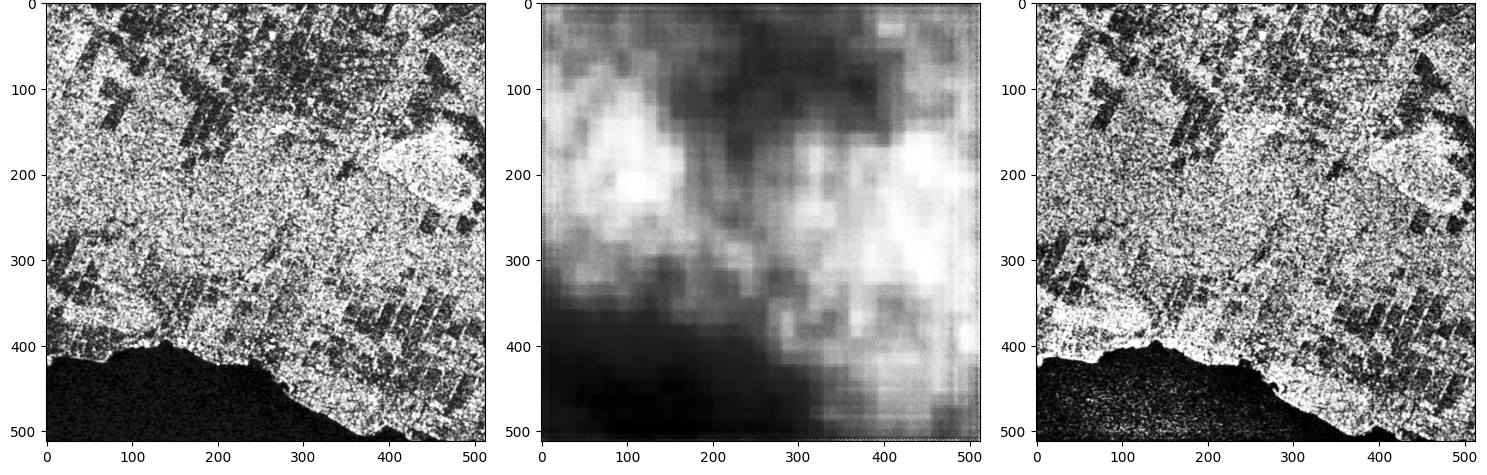
\includegraphics[width=0.85\textwidth]{Images/imratio_imreales_config1.png}
		\caption{Ejemplo para la configuración B1.}
		\label{fig:ratios_imreales_1}
	\end{subfigure}
	
	\vspace{0.5cm} % Espacio entre las subfiguras
	
	\begin{subfigure}[b]{\textwidth}
		\centering
		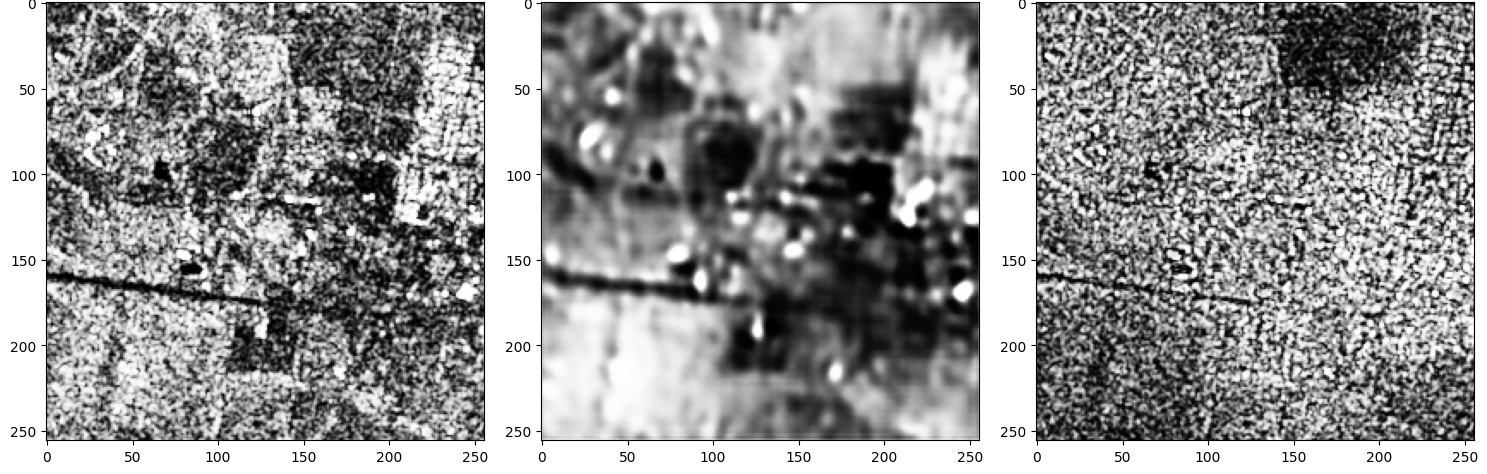
\includegraphics[width=0.85\textwidth]{Images/imratio_imreales_config3.png}
		\caption{Ejemplo para la configuración B3.}
		\label{fig:ratios_imreales_3}
	\end{subfigure}
	
	\vspace{0.5cm} % Espacio entre las subfiguras
	
	\begin{subfigure}[b]{\textwidth}
		\centering
		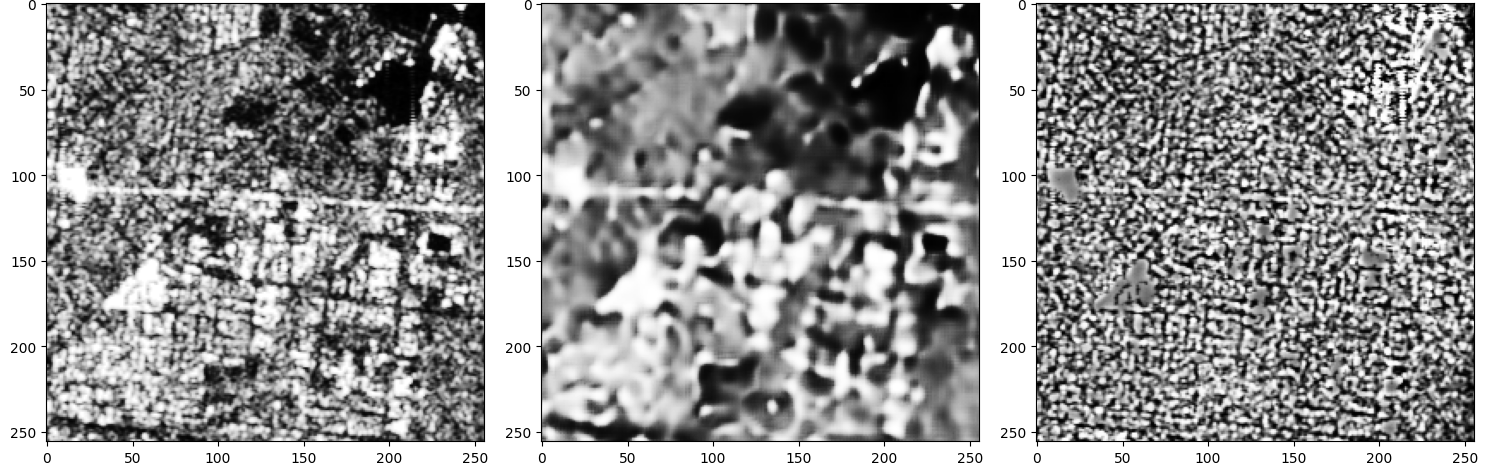
\includegraphics[width=0.85\textwidth]{Images/imratio_imreales_config5.png}
		\caption{Ejemplo para la configuración B5.}
		\label{fig:ratios_imreales_5}
	\end{subfigure}
	
	\caption{Ejemplos de imágenes procesadas por distintos modelos entrenados con imágenes reales, junto con sus correspondientes imágenes ratio (original/procesada). A la izquierda siempre vemos la imágen original (ruidosa), en el centro la imagen de salida del modelo, y a la derecha la imagen ratio.}
	\label{fig:ratios_imreales}
\end{figure}

Podemos observar que el modelo B1, que presenta el peor desempeño según la métrica de test, también exhibe la peor imagen ratio: en ella se distinguen con claridad la mayoría de las estructuras originales, lo que indica que el filtrado fue insuficiente y la imagen está lejos de asemejarse a un patrón de ruido puro. En cambio, el modelo B3 logra un resultado intermedio: su imagen ratio pierde gran parte de las estructuras principales, aunque aún pueden identificarse ciertas zonas oscuras y la traza de rutas. Finalmente, el modelo B5, el mejor según la métrica de test, genera una imagen ratio mucho más próxima al comportamiento ideal, con un patrón que se aproxima al ruido puro. No obstante, todavía pueden distinguirse de manera muy tenue algunas estructuras finas, especialmente aquellas asociadas a detalles lineales como calles.

Para el cálculo del estadístico de primer orden, tal como indicamos en la Sección \ref{sec:train_real_images}, tomamos manualmente regiones oscuras de la imágen, que se corresponden con zonas homogéneas. En la Figura \ref{fig:cuadrado_rojo} se ve un ejemplo de una región seleccionada. Para cada filtro tomamos 3 imágenes, y en cada una de ella elegimos a su vez 3 zonas oscuras de $30\times30$ píxeles. En cuanto al estadístico de segundo orden, se calcula de forma sencilla ya que el procedimiento es el mismo que para los modelos entrenados con imágenes sintéticas.

\begin{figure}[htbp]
	\vspace{0.2cm}
	\centering
	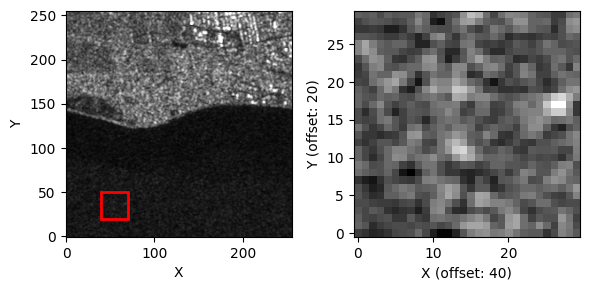
\includegraphics[height=5.6cm]{Images/cuadrado_rojo.png}
	\caption{Ejemplo de región oscura seleccionada manualmente utilizada para el cálculo del estadístico de primer orden. A la izquierda se ve la imagen original en donde se marca la zona elegida con un cuadrado rojo. A la derecha se ve un acercamiento a esa zona.}
	\label{fig:cuadrado_rojo}
\end{figure}

En la Tabla \ref{tab:statistics_results_imreales} presentamos los valores de los estadísticos de primer y segundo orden obtenidos. La suma de ambos, $\mathcal{M}$, se usa para ordenar los modelos. Si comparamos este ranking con el obtenido a partir del error de testeo (cuadro \ref{tab:testing_imreal_results}), observamos una correspondencia general entre ambos criterios: las configuraciónes B5 y B1 se mantienen dentro de las de mejor y peor desempeño respectivamente. Sin embargo, en este caso el ranking basado en los estadísticos ubica a la configuración B4 en primer lugar, desplazando a B5, que había mostrado el menor error de testeo.

Al igual que en los modelos entrenados con imágenes sintéticas, el estadístico de segundo orden ($\delta_h$) predomina sobre el de primer orden en la suma $\mathcal{M}$. No obstante, observamos que en este conjunto los valores de $\delta_h$ son considerablemente más altos que los obtenidos en el caso de entrenamiento con imágenes artificiales, mientras que los de $r_{\text{ENL},\mu}$ se mantienen en el mismo orden de magnitud. Esta diferencia sugiere que los modelos entrenados con imágenes reales logran un filtrado menos homogéneo, lo cual es esperable dado que dichas imágenes presentan una mayor complejidad estructural y variabilidad que las sintéticas.

\begin{table}[htbp]
	\hspace{0.2cm}
	\centering
	\caption{Resultados de los estadísticos de primer ($r_{\text{ENL},\mu}$) y segundo orden ($\delta_h$) para cada configuración entrenada con imágenes reales, junto con la suma de ambos ($\mathcal{M}$). Se ordenan de menor a mayor valor de $\mathcal{M}$.\newline}
	\label{tab:statistics_results_imreales}
	\small
	\begin{tabular}{|c|c|c|c|c|}
		\hline
		\textbf{Ranking} &
		\textbf{Config.} &
		\makecell{$r_{\text{ENL},\mu}$} &
		\makecell{$\delta_h$} &
		$\mathcal{M}$ \\
		\hline
		1 & B4 & 0.778 & 27.388 & 28.166 \\
		2 & B5 & 0.540 & 29.319 & 29.859 \\
		3 & B3 & 0.298 & 30.721 & 31.019 \\
		4 & B2 & 0.487 & 30.591 & 31.078 \\
		5 & B1 & 0.159 & 49.346 & 49.505 \\
		\hline
	\end{tabular}
	\vspace{0.5cm}
\end{table}

\titulito{Consideraciones finales}

Creemos importante destacar que estos modelos, entrenados con imágenes reales, muestran visualmente un mejor desempeño que aquellos entrenados con imágenes artificiales luego aplicados a imágenes reales. Sin embargo, reconocemos que los resultados aún no son perfectos. Estimamos que arquitecturas más profundas y un dataset de entrenamiento más amplio podrían contribuir significativamente a mejorar la calidad de las reconstrucciones, aunque las limitaciones de tiempo y recursos computacionales no nos permitieron realizar entrenamientos de tal envergadura.

También es importante notar que para estos experimentos utilizamos dimensiones de \emph{encoding} significativamente mayores que en los modelos entrenados con imágenes sintéticas. Esta decisión se justifica considerando que las imágenes reales son intrínsecamente mucho más complejas que las artificiales, y por tanto, deberían requerir una dimensión mayor para ser representadas adecuadamente en el espacio latente. Creemos que un espacio de \emph{encoding} aún mayor probablemente resultaría en mejores reconstrucciones, pero esto implicaría un número de parámetros entrenables que excede nuestras capacidades computacionales actuales para este trabajo.